\chapter{Variation und Wandel der Kasusrektion von Präpositionen im Deutschen} \label{cha:SekPraeps}
Ein Phänomen, das von Sprecher:innen des Deutschen stark reflektiert wird und auf das in zahlreichen Spracheinstellungsäußerungen Bezug genommen wird, sind die Variation und der Wandel im Bereich der Kasusrektion von Präpositionen. 
Zahlreiche Präpositionen des Deutschen können sowohl mit dem Genitiv als auch mit dem Dativ gebraucht werden: 

\begin{exe}
\ex Das war aus meiner Sicht nur \emph{während des} Studiums so. (DWDS, 2000, Die Zeit)\footnote{Alle \citeauthor{DWDS}-Belege stammen aus den aggregierten Referenz- und Zeitungskorpora von 2000 bis 2018.}
\ex Und \emph{während dem} Studium an der Wirtschaftshochschule wurden sie rot. (DWDS, 2017, Die Zeit)
\end{exe}
Die beiden Belege aus dem \citeauthor{DWDS} zeigen, dass die Präposition \waehrend{} sowohl mit dem Genitiv als auch mit dem Dativ gebraucht wird, ohne dass sich ein Unterschied in der Denotation ergeben würde. 
Dies grenzt die hier behandelten Dativ-Genitivschwankungen von Wechselpräpositionen ab, die zwischen Dativ und Akkusativ variieren und bei denen je nach Kasusrektion entweder eine Richtung (Akkusativ) oder eine Position (Dativ) denotiert wird.  
Einen Überblick über die Faktoren zu geben, die für die Variation zwischen Dativ- und Genitivrektion relevant sind, ist Ziel des folgenden Kapitels. 
Dafür ist es wichtig, zunächst einen Blick auf die grammatischen Eigenschaften von Präpositionen zu werfen. 
\autoref{sec:PraepDE} stellt daher die Wortart der Präpositionen im Deutschen vor (\autoref{sec:Wortart}) und erläutert die Einteilung in Primär- und Sekundärpräpositionen (\autoref{sec:Primaer} und \autoref{sec:Sekundaer}). 
Anschließend wird in \autoref{sec:Grammatikalisierung} auf die Entstehung und Entwicklung von Präpositionen im Rahmen der Grammatikalisierungstheorie eingegangen, wobei insbesondere die vier hier untersuchten Sekundärpräpositionen (\object{wegen, während, dank} und \object{gegenüber}) berücksichtigt werden. 
In \autoref{sec:LexikGrammatik} werden zunächst allgemeine Grammatikalisierungstendenzen der Präpositionen besprochen. 
Bei der anschließend thematisierten Kasusrektion lassen sich zwei Entwicklungstendenzen beobachten: die Entwicklung von der Genitiv- zur Dativrektion und die umgekehrte Entwicklung von der Dativ- zur Genitivrektion. 
Wie in \autoref{sec:Prototypisierung} und \autoref{sec:Differenzierung} gezeigt wird, kann insbesondere die Entwicklung zur Genitivrektion nicht allein durch voranschreitende Grammatikalisierung erklärt werden. 
In \autoref{sec:IndexikalitaetRektionskasus} geht es daher um die Indexikalität der Rektionsvarianten, die einen weiteren Erklärungsfaktor darstellt. 
Hier werden korpuslinguistische Distributionen (\autoref{sec:KorpusstudienRektion}), der Registrierungsprozess in Grammatiken und sprachpflegerischen Schriften (\autoref{sec:IndexikalitaetRektionskasushistorisch}) sowie erste Überlegungen zur Reflexion im laienlinguistischen Diskurs thematisiert (\autoref{sec:IndexikalitaetRektionskasusheute}). 
Letztere erscheinen aufgrund der in \autoref{cha:SprachideologienundSpracheinstellungen} diskutierten Zusammenhänge zwischen Sprachideologien und Sprachgebrauch besonders relevant, wurden bisher in der Forschung aber selten berücksichtigt, weshalb sich die vorliegende Studie ihrer näheren Untersuchung annimmt. 
\section{Das Präpositionalsystem des Deutschen} \label{sec:PraepDE}
Präpositionen zählen zu den häufigsten Wörtern des Deutschen \citep[s.][636--637]{Griehaber2009}. 
So ist \object{in} das am zweithäufigsten gebrauchte Wort nach den Formen des Definitartikels \citep[s.][]{InstitutfurDeutscheSprache2012}. 
Gleichzeitig existiert aber eine große Zahl sehr niedrigfrequenter Vertreter wie \object{einschließlich}. 
In Bezug auf die Frequenz herrscht innerhalb der Wortart also eine große Varianz. 
Die Angaben zur Gesamtanzahl der Präpositionen im Deutschen schwanken zwischen unter 30 und ein paar Hundert, was in der Schwierigkeit begründet liegt, die Präpositionen von anderen Wortarten abzugrenzen \citep[s.][262]{Lindqvist1994}. 
Ein weiterer Grund ist die Offenheit der Wortart für neue Vertreter (\cites[s.][526]{Eisenberg1979}[17]{Lehmann1992}[§1429]{Duden2022}[354]{Helbig.2017}; \autoref{sec:LexikGrammatik}).
Im folgenden Abschnitt werden die Kriterien thematisiert, die Präpositionen ausmachen. 
\subsection{Eigenschaften der Wortart Präposition} \label{sec:Wortart}
Präpositionen sind unflektierbare Funktionswörter.\footnote{Die sich zeigenden Ansätze von Flexion diskutiert \citet{Nubling2005}.} 
Sie bilden den Kopf einer Pr{\"a}positionalphrase und regieren den Kasus der darin eingebetteten Nominalphrase (\cites[s.][630]{Griehaber2009}[182]{Eisenberg.2013}). 
Im Deutschen sind Präpositionen ihrem Bezugswort in den meisten Fällen vorangestellt (\object{unter dem Tisch}).\footnote{Auch in zahlreichen weiteren germanischen Sprachen stehen Präpositionen typischerweise vor der Nominalphrase. In vielen anderen Sprachen wie etwa dem Koreanischen, dem Finnischen, dem Ungarischen oder dem Hindi dominieren hingegen die Postpositionen \citep[s.][]{Dryer2013}. 
Daneben gibt es einige wenige Sprachen mit Inpositionen (etwa Anindilyakwa und Tümpisa Shoshone): Hier wird ein Element in die Nominalphrase eingefügt~\citep[s.][]{Dryer2013}.}
Es gibt allerdings auch postponierte (\object{der Umwelt zuliebe}) oder zirkumponierte (\object{um der guten Laune willen}) Vertreter. 

Als Präpositionalkasus kommt im Deutschen typenmäßig am häufigsten der Genitiv vor (z.\,B. \object{abseits, jenseits}), dann der Dativ (z.\,B. \object{bei, mit}) und schließlich der Akkusativ (z.\,B. \object{gegen, wider}) (\cites[s. etwa][131--132]{Eroms1981}[638]{Griehaber2009}; vgl. dazu auch \autoref{sec:Primaer} und \autoref{sec:Sekundaer}). 
Einige Präpositionen können nicht nur Nominalphrasen regieren, sondern z.\,B. auch eine andere Präpositionalphrase (\object{das ist von vor dem Krieg}). 
Pr{\"a}positionen sind nicht satzgliedf{\"a}hig, das hei{\ss}t, sie k{\"o}nnen nicht alleine ein Satzglied bilden~\citep[s.][633]{Griehaber2009}.
Als Köpfe von Präpositionalphrasen können sie aber Teile verschiedener Satzglieder sein, etwa von Adverbialen (\object{die Tasse steht auf dem Tisch}) oder von Präpositionalobjekten (\object{sie wartet auf den ICE}). 

Semantisch gesehen bringen Präpositionen Beziehungen zum Ausdruck, die z.\,B. lokal, temporal oder kausal sein können (\cites[ausführlich dazu][]{Eroms1981}[s. außerdem][365--366]{Jung1980}[51--53, 55]{Rauh1990}). 
\begin{exe}
\ex Ein hübsches und stolzes Paar \emph{unter} dem Eiffelturm. (DWDS, 2008, Die Zeit)
\ex Für die Kunden einer Champagner-Firma lieferte von Klingenberg \emph{vor} Weihnachten Geschenksträuße. (DWDS, 2000, Die Zeit) 
\ex Bei tausenden Menschen an der Golfküste fiel \emph{wegen} des Unwetters der Strom aus. (DWDS, 2011, Die Zeit)
\end{exe}
%Pr{\"a}positionen haben also die Funktion, zwei Größen zueinander in ein Verh{\"a}ltnis zu setzen, etwa die Tasche und den Tisch in (4) (\cites[s.][145]{Buscha1984}[296]{Braunmueller1985}. 
Dabei können keineswegs nur Verhältnisse zwischen Nominalphrasen ausgedrückt werden, sondern bspw. auch ein Verh{\"a}ltnis zwischen einem Verb und einem Substantiv wie in \textit{sie liest w{\"a}hrend der Fahrt}~\citep[s.][41]{Romare.2004}.

Zwar können die bisher genannten Kriterien als Kerneigenschaften von Präpositionen angesehen werden, jedoch bilden die Präpositionen keine homogene Klasse.
Es fällt daher schwer, Kriterien zu definieren, die für alle ihre Vertreter gelten und sie scharf von anderen Wortarten, wie etwa den Konjunktionen, abzugrenzen \citep[s.][264]{Lindqvist1994}. 
So sind die Pr{\"a}position \textit{w{\"a}hrend }und die Konjunktion \textit{w{\"a}hrend }morphologisch und semantisch gleich und unterscheiden sich lediglich in syntaktischer Hinsicht~\citep[s.][39]{Romare.2004}.
%Ein größeres Problem stellen \object{als} und \object{wie} in Vergleichen dar. 
%Diese werden teils als Präpositionen, teils als Konjunktionen eingeordnet \citep[s.][41]{Romare.2004}.
%Von anderen nicht flektierbaren Wortarten sind Pr{\"a}positionen scheinbar recht leicht abgrenzbar, so weist \citet[129]{Eroms1981} darauf hin, die Abgrenzung von Interjektionen werde nicht diskutiert, da diese eine klare eigene Semantik aufwiesen. Er f{\"u}hrt jedoch an, dass bspw. das Kriterium der Kasusforderung auch bei einigen Interjektionen zu sehen sei (als Beispiel nennt er \object{weh mir})~\citep[s.][129]{Eroms1981}.

Ein Merkmal, das wie auch hier in der Literatur sehr h{\"a}ufig aufgef{\"u}hrt wird, ist die Unflektierbarkeit. 
\citet[10--11]{Lindqvist1994} weist jedoch darauf hin, dass dies in F{\"a}llen, in denen Partizipien pr{\"a}positional verwendet werden (bspw. \object{entsprechend}), problematisch sei, da es sich hierbei um flektierte Formen von Verben handele. 

Auch die wichtigste formale Eigenschaft der Präpositionen, die Rektion eines obliquen Kasus, entpuppt sich als nicht unproblematisch. 
So warnt \citet[29]{Lindqvist1994} davor, die M{\"o}glichkeit der Nominativrektion unber{\"u}cksichtigt zu lassen (\cites[s. auch][134]{Eroms1981}[695]{Engel1988}). 
Bei \object{je} bspw. wird davon ausgegangen, dass die Pr{\"a}position neben dem Akkusativ auch den Nominativ regieren kann~\citep[s.][291]{Hentschel1989}.\footnote{Teilweise werden außerdem Präpositionen ohne Kasusforderung angenommen \citep[so etwa bei][73]{Wunderlich1984}.}
\citet[291]{Hentschel1989} f{\"u}hrt zudem an, dass es wegen Synkretismusvermeidung h{\"a}ufig zur Nullflexion nach Pr{\"a}positionen kommt, wenn die Nominalphrase nur aus einem Substantiv ohne Erweiterung besteht (\textit{der Unterschied zwischen Affe und Mensch}). 

\citet{Lindqvist1994} vertritt die Auffassung, eine klare Abgrenzung der Pr{\"a}positionen von anderen Wortarten sei in vielen F{\"a}llen nicht m{\"o}glich.
%Hinweise auf die Schwierigkeit der Trennung finden sich auch etwa bei ,\citet[Quelle?]{Paul1920}, \citet[Quelle?]{Behagel1924} und \citet[Qualle?]{Braunmueller1982}. 
Statt einer starren Einteilung schl{\"a}gt er daher ein Modell vor, bei dem die infrage kommenden W{\"o}rter entlang einer Skala angeordnet werden~\citep[s.][5]{Lindqvist1994}. 
Auf diese Weise lässt sich zwischen prototypischen Vertretern der Wortart und peripheren Mitgliedern unterscheiden. 
Dieser Ansatz soll auch hier verfolgt und in den folgenden beiden Abschnitten näher erläutert werden. 
\subsection{Prototypische Präpositionen} \label{sec:Primaer}
Betrachtet man das Präpositionalsystem des Deutschen, lässt sich eine Gruppe prototypischer Präpositionen wie \object{in}, \object{auf}, oder \object{an} ausmachen, die den Kern der Wortart darstellt \citep[s.][214]{DiMeola2011}. 
Die Gruppe umfasst nur etwa 20 Mitglieder, die als Primärpräpositionen bezeichnet werden \citep[s.][94]{Szczepaniak2011}.\footnote{\citet[146]{Buscha1984} spricht von 40 Primärpräpositionen, die er allerdings nicht einzeln aufführt.}  
Als Prototyp lassen sich die Primärpräpositionen vor allem aufgrund ihrer hohen Frequenz auffassen (\cites[s.][631]{Griehaber2009}[94]{Szczepaniak2011}[§1429]{Duden2022}).
So gehören etwa die Primärpräpositionen \object{in, von} und \object{mit} zu den zehn häufigsten Wörtern des Deutschen \citep[s.][]{InstitutfurDeutscheSprache2012}. 
\autoref{table:FrequenzPraepositionen} listet die 20 Primärpräpositionen nach ihrer Frequenz laut der Wortgrundformenliste (DeReWo) des IDS auf sowie im Vergleich die Frequenz der vier in dieser Studie untersuchten Sekundärpräpositionen.
% Please add the following required packages to your document preamble:
% \usepackage{multirow}
% \usepackage[table,xcdraw]{xcolor}
% If you use beamer only pass "xcolor=table" option, i.e. \documentclass[xcolor=table]{beamer}
\begin{table}
\begin{tabular}{llr}
\lsptoprule
       & Präposition           & Häufigkeitsklasse \\\midrule
primär & \object{in}           & 2              \\
       & \object{von}          & 3              \\
       & \object{mit}          & 3              \\
       & \object{für}          & 4              \\
       & \object{auf}          & 4              \\
       & \object{zu}           & 4              \\
       & \object{an}           & 4              \\
       & \object{bei}          & 4              \\
       & \object{nach}         & 5              \\
       & \object{aus}          & 5              \\
       & \object{über}         & 6              \\
       & \object{vor}          & 6              \\
       & \object{durch}        & 6              \\
       & \object{gegen}        & 6              \\
       & \object{um}           & 6              \\
       & \object{bis}          & 6              \\
       & \object{zwischen}     & 7              \\
       & \object{seit}         & 7              \\
       & \object{ab}           & 7              \\
       & \object{unter}        & 7              \\\midrule
sekundär  & \object{wegen}     & 8              \\
          & \object{während}   & 8              \\
          & \object{gegenüber} & 9              \\
          & \object{dank}      & 11             \\
\lspbottomrule
\end{tabular}
\caption{Die 20 Primärpräpositionen und die vier hier untersuchten Sekundärpräpositionen nach Frequenz (Frequenzangaben aus \citealt{InstitutfurDeutscheSprache2012})}
\label{table:FrequenzPraepositionen}
\end{table}

Die Frequenzen in der Wortgrundformenliste basieren auf dem Deutschen Referenzkorpus (DeReKo) und werden in Häufigkeitsklassen angegeben: \glqq Dabei hat ein Wort die
Häufigkeitsklasse N, wenn das häufigste Wort etwa 2$^{N}$-mal häufiger vorkommt als dieses Wort\grqq{} \citep[13]{InstitutfurDeutscheSprache2012}. 
Das häufigste Wort sind die Determiniererformen \object{der}, \object{die} und \object{das}. 
Das zweithäufigste Wort, die Präposition \object{in}, kommt bereits nur noch um ein Vierfaches seltener vor.\footnote{Klitisierte Formen wie \object{im} sind in der Wortgrundformenliste gesondert aufgeführt, werden hier aber nicht mit aufgenommen.} 
Hier zeigt sich die für Häufigkeitsverteilungen in der Sprache typische Zipf-Kurve: Nur wenige Präpositionen kommen sehr häufig vor, während die große Mehrzahl der Präpositionen selten ist \citep[s.][22--27]{Zipf.1972}.

Bei den Primärpräpositionen handelt es sich nicht nur um die frequentesten, sondern auch um die ältesten Vertreter der Wortart. 
Sie werden bereits seit dem Althochdeutschen gebraucht~\citep[s.][1]{Graff.1824}.
Ein weiterer Hinweis auf den Charakter der Primärpräpositionen als prototypische Vertreter der Wortart ist ihr früher Erwerb \citep[s.][203--206]{Becker2011}. 

\begin{sloppypar}
Neben diesen prototypischen Primärpräpositionen finden sich sprachhistorisch neue Präpositionen, die Sekundärpräpositionen.
Zu dieser Gruppe gehören die hier untersuchten Präpositionen \object{dank}, \object{wegen}, \object{während} und \object{gegenüber}. 
Sekund{\"a}rpr{\"a}positionen sind im Vergleich zu Prim{\"a}rpr{\"a}positionen deutlich weniger tokenfrequent~\citep[636--637]{Griehaber2009}.
\object{Wegen} ist unter den Sekundärpräpositionen eine der häufigsten und steht in der DeReWo-Wortgrundformenliste auf Platz acht, zusammen mit Wortformen wie \object{Haus} und \object{ihm} \citep[s.][]{InstitutfurDeutscheSprache2012}. 
Die Gruppe hat aber eine große Anzahl an Vertretern, ist also sehr viel typenfrequenter \citep[s.][93]{Szczepaniak2011}.
\end{sloppypar}

Von den Sekundärpräpositionen lassen sich noch einmal die Tertiärpräpositionen unterschieden \citep[s.][631]{Griehaber2009}. 
Hierbei handelt es sich um Einheiten, die aufgrund ihres peripheren Status als Präpositionen in Verbindung mit einer Primärpräposition stehen müssen, über die sie den Kasus einer Nominalphrase regieren, wie \object {im Hinblick auf} oder \object{in Verbindung mit}. 
Mit dieser Primärpräposition zusammen bilden sie dann eine neue präpositional verwendete Einheit.\largerpage[1.5]

Prim{\"a}r-, Sekund{\"a}r- und Tertiärpr{\"a}positionen stellen keine distinkten Gruppen dar, sondern sollten, wie \citet[261]{Lindqvist1994} in seiner Untersuchung zu Präpositionen im Deutschen und Schwedischen argumentiert, als Kontinuum gesehen werden.\footnote{\citet[18--21]{Lindqvist1994} merkt an, dass die Darstellung anhand einer Skala nicht implizieren soll, dass allen Parametern tats{\"a}chlich nat{\"u}rliche Skalen zugrunde liegen. 
So l{\"a}sst sich etwa der Wechsel von der Nach- zur Voranstellung nur als skalare Ver{\"a}nderung auffassen, wenn der Bezugspunkt der idealisierte Prototyp einer Präposition ist.
Zudem können innerhalb der einzelnen Parameter Ver{\"a}nderungen durchaus sprunghaft stattfinden. Manche Parameter wie etwa die L{\"a}nge einer Pr{\"a}position lassen sich zwar kontinuierlich darstellen, dabei ist aber zu beachten, dass es sich dennoch nicht um kontinuierliche Prozesse handelt, sondern der Wandel in kleinen Spr{\"u}ngen stattfindet.}
Das Pr{\"a}positionalsystem ist also prototypisch organisiert~\citep[s.][33--34]{Bene.1975}. 

Auch nach außen hin sind Präpositionen kaum klar abgrenzbar, wie in \autoref{sec:Wortart} bereits angeklungen ist. 
Daher schlagen bereits \citet{Quirk.1964} vor, keine scharfe Abgrenzung von Pr{\"a}positionen und anderen Wortarten vorzunehmen. 
Auf diese Weise geht auch \citet[]{Lindqvist1994} vor: Er fragt nicht danach, ob eine Einheit eine Präposition ist oder nicht, sondern verfolgt einen Prototypenansatz, indem er danach fragt, wie nah die Einheit an der prototypischen Präposition ist \citep[s.][13]{Lindqvist1994}. 
Hierfür definiert er ein sogenanntes Idealpräpositionale, also das Ideal\-modell einer Pr{\"a}position \citep[s.][15--16]{Lindqvist1994}. 
Dieses Idealpräpositionale weist Eigenschaften auf, die prototypische Vertreter der Präpositionen in der Regel teilen. 
Dazu geh{\"o}ren sowohl formale als auch funktionale Eigenschaften. 
Auf der formalen Seite sticht vor allem die Kürze ins Auge: Prototypische Präpositionen sind meistens einsilbig und haben eine simple Silbenstruktur \citep[s.][§1430]{Duden2022}. 
Ausnahmen wie \object{über} und \object{unter} weichen von dieser Einsilbigkeit ab und stehen dem Prototyp somit weniger nah als \object{auf} oder \object{mit}.
Mit ihrer Kürze hängt eng zusammen, dass Primärpräpositionen morphologisch nicht segmentierbar sind \citep[s.][33]{Lehmann1992}. 
Wie oben bereits erwähnt, gehört auch die Voranstellung zu den prototypischen Eigenschaften.  
Eine wesentliche funktionale Eigenschaft prototypischer Präpositionen ist die semantische Vielwertigkeit \citep[s.][15]{Lindqvist1994}. 
Primärpräpositionen können oft neben einer konkreten lokalen Bedeutung sehr abstrakte grammatische Bedeutungen haben (\object{auf dem Tisch stehen} vs. \object{auf den Bus warten}).\footnote{\citet[10--11]{Lehmann1992} unterscheiden innerhalb der Primärpräpositionen noch eine weitere Gruppe, nämlich grammatische Präpositionen wie \object{von} und \object{zu}.}
Auch syntaktisch sind Primärpräpositionen vielwertig.
Bspw. können sie zum Teil als Verbpartikeln (\textit{aufessen, anschalten, mitgehen}) und in Pronominaladverbien (\textit{darauf, darin}) auftreten~\citep[s.][275--276]{Lindqvist1994}.  
Zudem können Prim{\"a}rpr{\"a}positionen selbst regiert werden von Substantiven (\textit{Glaube an}), Adjektiven (\textit{reich an}), komplexen Pr{\"a}positionen (\textit{mithilfe von}) oder als Einleiter von Präpositionalobjekten von Verben (\textit{warten auf}) \parencites[s.][39]{Lehmann1992}[68]{Diewald.1997}.

Die für die vorliegende Untersuchung wichtigste Eigenschaft der Präpositionen ist ihr Rektionskasus. 
Dieser ist bei den Primärpräpositionen der Dativ oder der Akkusativ \citep[s.][94]{Szczepaniak2011}. 
Eine besondere Gruppe innerhalb der Primärpräpositionen bilden die Wechselpräpositionen \object{in, auf, an, über, vor, unter, zwischen, neben, hinter} (\citealp[s.][§1439--1441]{Duden2022}, hier geordnet nach der Frequenz in einer Korpusuntersuchung im LIMAS-Korpus von~\citealp[19]{Folsom1984}). 
In der Regel gilt für die Wechselpräpositionen, dass sie den Dativ regieren, wenn auf eine statische Position referiert wird, während sie den Akkusativ regieren, wenn eine Richtungsbewegung beschrieben wird \citep[s.][§1439]{Duden2022}. 
\begin{exe}
\ex \ExampleFont{Er hätte \emph{auf dem} Podest stehen können.} (DWDS, 2005, Berliner Zeitung) 
\ex \ExampleFont{Erstmals in dieser Saison \emph{auf das} Podest schaffte es der Tscheche Lukas Hlava als Dritter.} (DWDS, 2012, Die Zeit)
\end{exe}
Wenn in dieser Studie von Rektionsvarianten gesprochen wird, sind die verschiedenen Rektionsmöglichkeiten der Wechselpräpositionen nicht gemeint, da diese Möglichkeiten semantisch gesteuert sind \citep[s.][703]{Engel1988}.
\subsection{Peripherie der Wortart}
\label{sec:Sekundaer}
Nachdem nun die prototypischen Vertreter der Wortart Präposition vorgestellt wurden, wird im folgenden Abschnitt auf die Peripherie der Wortart eingegangen, insbesondere auf die Gruppe der Sekundärpräpositionen. 
Sekundärpräpositionen sind sprachhistorisch jünger als Primärpräpositionen. 
In einer Korpusuntersuchung zu Präpositionen im Mittelhochdeutschen von \citet[]{Waldenberger.2009} kommt keine der hier untersuchten Pr{\"a}positionen \object{wegen}, \object{während}, \object{dank} und \object{gegenüber} vor. 
Wann genau die Entwicklung komplexer Pr{\"a}positionen begonnen hat, ist unklar, vermutet wird aber, dass dies im Fr{\"u}hneuhochdeutschen der Fall war~\citep[s.][50]{Meibauer1995}. 
\citet[43]{Romare.2004} geht davon aus, dass Sekundärpräpositionen ab dem Sp{\"a}tmittelalter entstehen. 

Sekundärpräpositionen verfügen im Vergleich mit Primärpräpositionen über eine spezifischere eigene Semantik, die aber bereits zu verblassen beginnt (\autoref{sec:LexikGrammatik}). 
So lässt sich etwa die Bedeutung von \object{einschließlich} genauer umschreiben als die von \object{in}. 
\citet[42--43]{Bene.1975} f{\"u}hrt daher die explizitere Beschreibung der Relation als einen Grund f{\"u}r die Verwendung neuer Pr{\"a}positionen an. 
Laut \citet[67]{Diewald.1997} beschreiben sie Relationen, {\glqq}die übereinzelsprachlich gesehen selten oder nie vollst{\"a}ndig grammatikalisiert werden{\grqq}. 
\citet{Eisenberg1979} pl{\"a}diert aufgrund ihrer konkreten Semantik f{\"u}r einen lexikalischen Status der morphologisch komplexen Pr{\"a}positionen.

Auf formaler Seite unterscheiden sich die Sekundärpräpositionen von den Primärpräpositionen insbesondere dadurch, dass sie sich in mehrere Morpheme zerlegen lassen oder zumindest morphologisch transparent sind \citep[s.][62]{DiMeola2001}. 
So weist \object{mithilfe} die Morpheme \{mit\} und \{hilfe\} auf. 
Auch \object{während} ist segmentierbar (\{währen\} + \{d\}). 
Sekundärpräpositionen wie \object{dank} oder \object{trotz} lassen sich zwar nicht weiter segmentieren, weisen aber morphologische Transparenz auf, da sie mit Substantiven oder Verbstämmen identisch sind, aus denen sie sich entwickelt haben. 

Während die Primärpräpositionen vorangestellt werden, gibt es unter den Sekundärpräpositionen einige Vertreter, die nachgestellt oder zirkumponiert sind \citep[s.][152]{DiMeola2000}.
\begin{exe}
\ex \ExampleFont{Erlaubt waren dabei dem Regelwerk \emph{entsprechend} 100 Kilometer.} (DWDS, 2012, Die Zeit)
\ex \ExampleFont{Familienpolitik muss aber \emph{um} der Kinder \emph{willen} gemacht werden.} (DWDS, 2002, Berliner Zeitung)
\end{exe}
Zudem variieren einige Sekundärpräpositionen zwischen Voran- und Nachstellung oder sogar zwischen Voran-, Nach- und Zirkumstellung, etwa (\object{von}) \object{wegen}. 
\begin{exe}
\sloppy
\ex \ExampleFont{Insgesamt fielen \emph{wegen} des Streiks mehr als 1500 Flüge aus.} (DWDS, 2012, Die Zeit)
\ex \ExampleFont{Die besten unserer Amtsträger kandidieren nicht des Geldes \emph{wegen}.} (DWDS, 2013, Die Zeit) 
\ex \ExampleFont{Deshalb gehört solchen Tendenzen \emph{von} Gesetzes \emph{wegen} ein Riegel vorgeschoben.} (DWDS, 2000, Der Tagesspiegel)
\end{exe}
In den syntaktischen Funktionen, die sie ausfüllen können, sind die Sekundärpräpositionen eingeschränkter als die Primärpräpositionen, da sie keine Präpositionalobjekte einleiten können. 
Anders als mit Primärpräpositionen können mit Sekundärpräpositionen außerdem keine Pronominaladverbien gebildet werden \citep[s.][526]{Eisenberg1979}:
\object{damit}, \object{dabei} usw., aber *\object{dawährend}.

%\begin{quote}W{\"a}hrend die morphologisch einfachen (alten) Pr{\"a}positionen Proforrnen mit pr{\"a}figierten \textit{da(r) (davor, darin) }bilden, ben{\"o}tigen die morphologisch komplexen den nachgestellten Genitiv des Relativpronomens \textit{(infolge dessen, anhand deren).}~\citep[526]{Eisenberg1979}\end{quote}
Betrachtet man die Kasusrektion der Sekundärpräpositionen, so fällt auf, dass hier neben der Dativ- und der Akkusativrektion auch die Genitivrektion möglich ist.\footnote{Daneben kommen Präpositionen vor, die keinen bestimmten Kasus regieren, also mit allen Kasus auftreten können, wie etwa \object{minus} (\cites[40--41]{Lindqvist1994}[§1452]{Duden2022}). Ob Einheiten wie \object{minus} oder \object{plus} zu den Präpositionen gerechnet werden sollten, ist fraglich, soll hier jedoch nicht weiter diskutiert werden.} 
Der Genitiv ist unter den Sekundärpräpositionen sogar der am häufigsten regierte Kasus \citep[s.][16]{Lehmann1992}. 
Aufgrund der hohen Typenfrequenz der Sekundärpräpositionen hat die Genitivrektion damit insgesamt die höchste Typenfrequenz unter den Präpositionen (\cites[s.][131--132]{Eroms1981}[638]{Griehaber2009}). 
Sehr häufig variieren die Sekundärpräpositionen in ihrer Kasusrektion, meist zwischen Genitiv und Dativ (\cites[s.][§1449--1451]{Duden2022}[zu Schwankungen bei historisch neuen Akkusativpr{\"a}positionen wie etwa \textit{pro} s.][]{Hentschel1989}). 
\citet[32]{Lindqvist1994} nennt ca. 40~Pr{\"a}positionen, die ausschlie{\ss}lich den Genitiv regieren können und keine Variation aufweisen (etwa \textit{bar, zuz{\"u}glich, kraft, im Laufe}). 
Für die meisten Sekundärpräpositionen, auch für einige der von \citet{Lindqvist1994} genannten, lassen sich jedoch Belege für verschiedene Rektionsvarianten finden, wie \citeauthor[]{DiMeola2000} in Korpusuntersuchungen zeigt (s. etwa \citeyear[]{DiMeola1999, DiMeola2000, DiMeola2006}). 
Anders als bei den Wechselpräpositionen ist diese Variation nicht im engeren Sinne semantisch gesteuert, d.\,h. es gibt auf der denotativen Ebene keinen Unterschied zwischen Varianten wie \object{während des Studiums} und \object{während dem Studium}. 
Der \citet[]{Duden2022} schreibt dazu: 
\begin{quote}Bei vielen Präpositionen schwankt die Rektion zwischen zwei (oder sogar mehr) Kasus, ohne dass damit eine Bedeutungsveränderung einhergeht. Häufig gibt es regionale oder Registerunterschiede etwa zwischen Umgangssprache und gehobener 
Sprache oder mündlichem und schriftlichem Sprachgebrauch.~\citep[{\S}1448]{Duden2022}\end{quote}
%\begin{quote}Einige Pr{\"a}positionen schwanken in ihrer Rektion, ohne dass dies Einfluss auf ihre Bedeutung h{\"a}tte. Hier vollzieht sich Sprachwandel (man spricht von Nebenkasus): \object{wegen des Geldes (Genitiv) / wegen dem Geld (Dativ); dank ihres Einsatzes / dank ihrem Einsatz}~\citep[{\S}910]{Duden2016}\end{quote}
Dass beide Varianten von Sprachbenutzer:innen zudem sehr unterschiedlich bewertet werden, ist Thema dieser Studie und wird in \autoref{sec:IndexikalitaetRektionskasusheute} näher beleuchtet. 
In einigen Fällen wird die Dativrektion auch durch die syntaktische Umgebung begünstigt. 
So kommt der Dativ bspw. häufig vor, wenn sonst zwei Genitivphrasen aufeinanderfolgen würden (\object{während dem Korrigieren des Buchs} oder \object{während Tims langem Aufenthalt}). Folgt ein Substantiv ohne Determinierer auf die Präposition, bleibt es häufig endungslos (\object{wegen Umbau}) \citep[s.][§1450--1451]{Duden2022}. 

\autoref{table:Kontinuum} zeigt zusammenfassend die besprochenen formalen und funktionalen Unterschiede zwischen Primär- und Sekundärpräpositionen und führt daneben auch die Eigenschaften der Tertiärpräpositionen auf. 
\begin{table}
\begin{small}
\centering
\begin{tabular}{lcrll}
\lsptoprule
 \textcolor{gray}{Tertiärpräpositionen}           & \ Sekundärpräpositionen \                                            & Primärpräpositionen                     \\
 \midrule
\textcolor{gray}{Rektion über} & Genitivrektion überwiegt, & Dat.- und/oder Akk.-\\\textcolor{gray}{Primärpräposition} &aber auch Dat.- oder & Rektion\\&Akk.-Rektion         \\
\textcolor{gray}{} &  &  \\\textcolor{gray}{prä-, zirkum-} & Stellung schwankt,& präponiert, \\
\textcolor{gray}{oder postponiert,}                  & mehr- oder einsilbig,                                            & einsilbig,                               \\
\textcolor{gray}{mehrsilbig,} \ \           & \ \ morphologisch segmentierbar \ \                                       & morphologisch nicht \\ \textcolor{gray}{morphologisch komplex},& oder transparent, & weiter unterteilbar,  \\
\textcolor{gray}{eher lexikalische}    & Semantik verblasst,                                              & eher grammatische \\\textcolor{gray}{Bedeutung,}   & mehr synt. Funktionen &Bedeutung,        \\
\textcolor{gray}{synt. Funktionen} &  & vielfältige synt. \\ \textcolor{gray}{eingeschränkt} & & Funktionen\\
\lspbottomrule
\end{tabular}
\end{small}
\caption{Formale und funktionale Eigenschaften von Primär-, Sekundär- und Tertiärpräpositionen}
\label{table:Kontinuum}
\end{table}

%Die Frage, ob es sich bei den Pr{\"a}positionen um eine offene oder geschlossene Wortklasse handelt, lässt sich also nicht für die gesamte Wortart beantworten, da zwischen den verschiedenen Typen von Präpositionen unterschieden werden muss \citep[s.][523]{Eisenberg1979}. 
%Insbesondere in früheren Arbeiten wurde von der Geschlossenheit der Wortart ausgegangen \citep[s. z.\,B.][]{Langacker1968}. 
%Im Strukturalismus wurden Pr{\"a}positionen als geschlossene Klasse eingeordnet, wofür laut \citet[34]{Rauh1990} insbesondere drei Argumente herangezogen wurden: \glqq 1. Präpositionen sind Funktions- oder Strukturwörter, 2. Präpositionen haben geringe lexikalische Bedeutung, 3. Die Menge der Präpositionen ist begrenzt und zeigt in einer Sprache diachronisch kaum Veränderungen.\grqq{} 
%Zu letzterem Argument führt sie an: {\glqq}Offensichtlich sind solche {\"A}u{\ss}erungen allein unter Ber{\"u}cksichtigung der in der Tag {\"u}berschaubaren Menge von urspr{\"u}nglichen oder prim{\"a}ren Pr{\"a}positionen gemacht worden{\grqq}~\citep[42]{Rauh1990}.
%\citet{Rauh1990} zeigt an Präpositionen des Englischen beispielhaft, dass diese Argumentation und demzufolge auch die Einteilung als geschlossene Klasse unangemessen ist und spricht selbst von einer \glqq potentiell unendlichen Menge von Präpositionen\grqq{}~\citep[55]{Rauh1990}. 
%Auch \citet[148]{Vestegaard.1973} sieht die Präpositionen im Englischen als produktiv an.\\ 
%Im Deutschen zeigt sich die Produktivität etwa darin, dass die Gruppe der Präpositionen Lehnwörter zulässt (\object{pro, via, versus} etc.) \citep[s.][197]{DiMeola2009}. 
%Auch die Verschmelzung von Pr{\"a}position und Substantiv, wie etwa bei \textit{mit Hilfe/mithilfe }zu beobachten, ist ein produktives Muster~\citep[s.][520]{Eisenberg1979}.  
%\citet{Eisenberg1979} stellt die Frage, warum die Gruppe der Pr{\"a}positionen st{\"a}ndig erweitert wird. 
%Den von ihm konstatierten zunehmenden Gebrauch von Pr{\"a}positionalobjekten sieht er nicht als Grund, da keine Sekund{\"a}r- oder Terti{\"a}rpr{\"a}position ein Pr{\"a}positionalobjekt einleiten k{\"o}nne \citep[524]{Eisenberg1979}.
Wie oben bereits erwähnt, handelt es sich bei den Sekundärpräpositionen (wie auch bei den Tertiärpräpositionen) um eine offene Klasse, die neue Vertreter aufnehmen kann. 
Das folgende Kapitel behandelt die Entstehung neuer Präpositionen und ihre Entwicklung insbesondere bezüglich der Kasusrektion. 
%\citet[]{Bene.1975} sieht folgenden Grund für das Hinzukommen neuer Sekundär- und Tertiärpräpositionen (bei ihm Halbpräpositionen): 
%\begin{quote}Die Halbpr{\"a}positionen bereichern das Inventar der modernen Schriftsprache. Der Hauptgrund, weshalb sich ihr Repertoire in der neueren Zeit st{\"a}ndig erweitert und erneuert, liegt wohl in ihrer semantischen Pr{\"a}gnanz.~\citep[44]{Bene.1975}\end{quote}
%Sekundär- und Tertiärpräpositionen können also als expressiver gelten, was ihre Verwendung in bestimmten Kontexten begünstigt \citep[s.][102]{Szczepaniak2011}. 
%Der Wunsch nach Expressivität kann als Motor für Sprachwandel angesehen werden uns stößt auch im Bereich der Präpositionen Grammatikalisierungsprozesse an \citep[s.][103]{Szczepaniak2011}.
%Diese Prozesse sind Thema des folgenden Kapitels. 
\section{Grammatikalisierung der Präpositionen}\label{sec:Grammatikalisierung}
In \autoref{sec:Primaer} und \autoref{sec:Sekundaer} wurden historisch alte Primärpräpositionen und historisch neue Sekundärpräpositionen aus synchroner Perspektive gegenübergestellt. 
In den folgenden beiden Abschnitten wird nun ein diachroner Blick eingenommen, der darauf abzielt, die bereits angesprochene synchron zu beobachtende Variation im Bereich der Rektion vor dem Hintergrund der historischen Entwicklung der Präpositionen zu beleuchten.

Mit Fragen des Sprachwandels im Bereich der Präpositionen haben sich bisher vor allem zahlreiche Arbeiten im Rahmen der Grammatikalisierungstheorie beschäftigt \citep[etwa][]{Lehmann1992, Lindqvist1994,  DiMeola2000, Szczepaniak2011}. 
Inwiefern sich die Entwicklungen der Präpositionen im Deutschen mithilfe der Grammatikalisierungstheorie erklären lassen, wird im Folgenden erörtert. \autoref{sec:LexikGrammatik} gibt zunächst einen Überblick über die bei der Grammatikalisierung ablaufenden Prozesse. 
\autoref{sec:Prototypisierung} und \autoref{sec:Differenzierung} widmen sich zwei Erklärungsansätzen für die Wandeltendenzen im Bereich der Rektion, wobei vor allem auf die Entwicklung der vier hier behandelten Sekundärpräpositionen \object{wegen}, \object{während}, \object{dank} und \object{gegenüber} eingegangen wird. 
Insbesondere die Arbeiten von \citeauthor{DiMeola2000} (v.\,a. \citeyear{DiMeola1998}, \citeyear{DiMeola2001}, \citeyear{DiMeola2001}, \citeyear{DiMeola2003},  \citeyear{DiMeola2004} und \citeyear{DiMeola2011}) sind dabei von Relevanz.  
\subsection{Von der Lexik in die Grammatik}
\label{sec:LexikGrammatik}
Die Grammatikalisierung eines sprachlichen Zeichens ist seine Entwicklung von einem (eher) lexikalischen Zeichen zu einem (eher) grammatischen oder von einem weniger grammatischen zu einem stärker grammatischen (\cites[s.][303]{Lehmann.1985}[193]{Lehmann.1991}[2]{Heine.1991}). 
Der Übergang zu einem grammatischen Zeichen geschieht nicht abrupt, sondern lässt sich mit dem Muster A>A/B>B modellieren (\cites[s.][107]{Heine.1991}[15]{Lehmann.1995}). 
Das heißt, in einer Übergangsphase kommt es auf funktionaler wie auf formaler Seite zu Variation. 
Dies zeigt sich auch bei den Sekundärpräpositionen, die etwa in ihrer Kasusrektion variieren (\autoref{sec:Sekundaer}). 

Präpositionen können zu den grammatischen Zeichen gezählt werden, da sie eine relationale Bedeutung haben \citep[s.][93]{Szczepaniak2011}. 
Dennoch werden sie von einigen als lexikalische oder teilweise lexikalische Zeichen gesehen. 
Für \citet[2076]{Zifonun1997} etwa handelt es sich bei Präpositionen um lexikalische Zeichen: \glqq W{\"a}ren Pr{\"a}positionen nur grammatisch-strukturelle Morpheme, so w{\"a}re die Offenheit der Klasse kaum zu erkl{\"a}ren\grqq. 
Auch \cite{Rauh1990} plädiert für den lexikalischen Status. 
\citet[182]{Eisenberg.2013} sieht die morphologisch komplexen Pr{\"a}positionen als lexikalisch an \citep[s. auch][]{Eisenberg1979}. 
\citet[136]{Eroms1981} schreibt Präpositionen sowohl einen grammatischen als auch einen lexikalischen Bedeutungsanteil zu.
\citet[42]{Romare.2004} sieht die Präpositionen zwar insgesamt als grammatische Klasse, bezeichnet ihre Funktion aber teils als lexikalisch, indem sie z.\,B. r{\"a}umliche Bedeutungen als lexikalisch einordnet, die Einleitung von Pr{\"a}positionalobjekten hingegen als grammatisch.
Die vorliegende Studie schließt sich der Grammatikalisierungsforschung an und betrachtet Präpositionen aufgrund ihrer relationalen Bedeutung als grammatische Zeichen. 
Dabei ist auch hier von einem Kontinuum auszugehen: Mit \citet[16, 306]{Lindqvist1994} lässt sich festhalten, dass typische Präpositionen eher grammatische Bedeutung haben, während untypische Präpositionen auch lexikalisch sein können.   
Auch die von einigen als lexikalisch eingeordnete lokale Bedeutung kann als grammatisch aufgefasst werden, was sich mit der Existenz lokativer Kasus in Sprachen wie dem Türkischen oder dem Lateinischen begründen lässt. 

Während Sprachbenutzer:innen beim Gebrauch lexikalischer Zeichen recht frei sind, unterliegt der Gebrauch grammatischer Zeichen festeren Regeln. 
So kann in dem Satz \object{das Kaninchen hoppelt/hüpft/rennt über das Feld} je nach Intention zwischen den unterschiedlichen Verben gewählt werden, wohingegen die Verbendung für die dritte Person Singular obligatorisch ist.  
Die Grammatikalisierung eines Zeichens wird von \citet[130]{Lehmann.1995} daher als der Verlust an Autonomie gefasst: 
Sowohl auf der paradigmatischen Ebene als auch auf der syntagmatischen Ebene wird ein Zeichen im Laufe seiner Grammatikalisierung weniger eigenständig. 
Um dies systematisch zu beschreiben, entwickelt \citet[305]{Lehmann.1985} die drei Grammatikalisierungsparameter Gewicht, Kohäsion und Variabilität. 
Bei jedem Parameter wird zwischen paradigmatischen und syntagmatischen Aspekten unterschieden \citep[s.][131]{Lehmann.1995}. 
\autoref{table:Grammatikalisierungsparameter}  bietet eine Übersicht über die Lehmannschen Grammatikalisierungsparameter, die nun der Reihe nach vorgestellt werden.  
\begin{table}
\centering
\begin{tabular}{lccr}
\lsptoprule
                 & paradimatisch & syntagmatisch  & \\
                 \midrule
Gewicht     & Integrität           & struktureller Skopus & (nimmt ab) \\
Kohäsion   &   Paradigmatizität   &  Fügungsenge & (nimmt zu) \\
Variabilität  & Wahlfreiheit        & Stellungsfreiheit  & (nimmt ab)\\
\lspbottomrule
\end{tabular}
\caption{Grammatikalisierungsparameter nach \citet[132]{Lehmann.1995}}
\label{table:Grammatikalisierungsparameter}
\end{table}

Der Parameter Gewicht wird von \citet[]{Lehmann.1985} auf paradigmatischer Ebene als Integrität eines Zeichens bezeichnet, auf syntagmatischer Ebene als struktureller Skopus. 
Die Integrität, also das paradigmatische Gewicht eines Zeichens, betrifft sowohl seine funktionale Seite als auch seine formale Seite \citep[s.][305]{Lehmann.1985}: Die Semantizität und die Länge eines Zeichens nehmen im Laufe der Grammatikalisierung ab. 
Wie oben bereits erwähnt (\autoref{sec:Sekundaer}) bilden die Präpositionen eine relativ offene Wortart, die gut neue Vertreter aufnehmen kann \citep[518]{Eisenberg1979}. 
Neue Präpositionen können aus Adjektiven (\object{zuzüglich}), Adverbien (\object{links}), Partizipien (\object{entsprechend}), Substantiven (\object{kraft}) oder auch aus Präpositionalphrasen (\object{aufgrund}) entstehen (\cites[s.][66]{DiMeola2001}[215]{DiMeola2011}; vgl. auch \citealp{Braunmueller1985}).
Insbesondere Substantive und Verben sind auch sprach{\"u}bergreifend typische Spenderbereiche f{\"u}r Pr{\"a}positionen (\cites[672]{Kortmann.1992}[512]{Konig.2012}). 
Am Beginn des Entwicklungsprozesses stehen also lexikalische Einheiten. 
Historisch neue Präpositionen, die aus diesen Einheiten entstehen, verfügen daher zunächst über eine recht spezifische Semantik. 
Im Gegensatz dazu erfüllen historisch alte, prototypische Präpositionen wie \object{auf} oft {\"a}hnliche Funktionen wie Kasus (\cite[s.][45]{Rauh1990}; \autoref{sec:Primaer}). 
Besonders deutlich ist dies bei der Präposition \object{von} zu sehen, die häufig anstelle eines Genitivs vorkommt (\object{das Buch von Johanna}) und sich damit in Richtung eines Kasusmarkers entwickelt \citep[s.][6]{Lehmann1992}. 
Auf der funktionalen Seite lässt sich also ein Verlust an Semantik ausmachen, der als Desemantisierung bezeichnet wird \citep[s.][493]{Lehmann.1991}.

%Präpositionen haben sowohl Eigenschaften lexikalischer Zeichen als auch Eigenschaften grammatischer Zeichen, weshalb die Einordnung in der Literatur unterschiedlich ausfällt.  Auch \citet[47]{Rauh1990} spricht davon, dass die Klasse der Pr{\"a}positionen heterogen sein und nicht als homogene Gruppe behandelt werden k{\"o}nne. \begin{quote}Viele Pr{\"a}positionen (so \object{beiderseits, innerhalb, kraft, namens, trotz}) haben eine eigene, leicht beschreibbare Bedeutung. Aber die am h{\"a}ufigsten gebrauchten Pr{\"a}positionen (\object{an, auf, durch, für, mit, nach, zu} und andere) haben je nach ihrer Verwendung unterschiedliche Bedeutungen, und in manchen F{\"a}llen haben sie {\"u}berhaupt keine beschreibbare Bedeutung [so \object{auf} in \object{Wir verlassen uns auf Sie.}).~\citep[691]{Engel1988}\end{quote}
Auch auf formaler Seite verlieren Zeichen im Laufe ihrer Grammatikalisierung an Gewicht (\cites[s.][16]{Heine.1991}[134]{Lehmann.1995}). 
Dieser Erosionsprozess führt dazu, dass Präpositionen kürzer werden, je stärker sie grammatikalisiert sind \citep[s.][66--67]{Diewald.1997}.
Dies ist bspw. bei \object{wegen} zu beobachten: Die Präposition kann im Gesprochenen bereits einsilbig vorkommen, indem sie nicht nur zu schwalosem [veːgŋ̩] verkürzt wird, sondern zu [veːŋ] \citep[s.][9]{Lindqvist1994}. 
Auch bei \gegenueber{} kann bei schnellem Sprechen bereits Erosion beobachtet werden ([geːgŋ̩yːbɐ]~> [geːŋyːbɐ]).

Der strukturelle Skopus nimmt bei der Entwicklung eines Wortes zu einer Pr{\"a}position ab. 
So erstreckt sich bspw. der Skopus des Adverbs \textit{gegenüber }auf die ganze Verbalphrase (s. \autoref{Bsp:ADVgeg}), w{\"a}hrend bei der Pr{\"a}position \textit{gegenüber }nur die Nominalphrase in ihrem Skopus liegt, wie \autoref{Bsp:APPRgeg} illustriert \citep[s.][301]{Braunmueller1985}:
\begin{exe}
\ex \ExampleFont{Mein Hotel lag draußen in einem Industriegebiet, \emph{gegenüber}} (ADV) \ExampleFont{konnte man Reifen, Baustahl und Heizöl kaufen} (DWDS, 2013, Zeit Magazin) \label{Bsp:ADVgeg}
\ex \ExampleFont{Der Bund muss verstehen, dass die Sparpolitik \emph{gegenüber}} (APPR) \ExampleFont{der Stiftung, mit der wir ja bereits Schluss gemacht haben, indem wir den Etat 2000 um 100 Millionen erhöht haben, nicht wiederaufgenommen werden kann.} (DWDS, 2000, Die Zeit) \label{Bsp:APPRgeg}
\end{exe}
Bei der paradigmatischen Kohäsion (Paradigmatizität) und der syntagmatischen Kohäsion (Fügungsenge) geht es darum, wie eng die Verbindung ist, die ein Zeichen mit anderen eingeht. 
Die Kohäsion nimmt im Laufe der Grammatikalisierung zu. 
F{\"u}r die Paradigmatizit{\"a}t ist die Gr{\"o}{\ss}e des Paradigmas, zu dem ein Zeichen geh{\"o}rt, entscheidend~\citep[141]{Lehmann.1995}. 
Ein weiterer Aspekt ist, wie homogen das Paradigma ist und wie systematisch die Unterschiede zwischen seinen einzelnen Elementen sind~\citep[143]{Lehmann.1995}. 
Wie in \autoref{sec:Sekundaer} dargestellt, sind die Sekundärpräpositionen eher lose zu einem sehr großen Paradigma organisiert, während die Primärpräpositionen ein kleineres, fester organisiertes Paradigma bilden \citep[s.][68]{Diewald.1997}. 
Die Primärpräpositionen können daher als geschlossene Klasse angesehen werden (\cites[s.][66]{Diewald.1997}[94]{Szczepaniak2011}[353]{Helbig.2017}).
Auch die Fügungsenge ist bei Primärpräpositionen größer als bei Sekundärpräpositionen. 
So können die am stärksten grammatikalisierten Primärpräpositionen mit dem Definitartikel verschmelzen, wie etwa \object{zum} oder \object{im} \citep[s.][]{Nubling2005}.

Die Variabilität bezieht sich darauf, inwiefern Sprachbenutzer:innen die Freiheit haben, ein Zeichen zu verwenden oder nicht, und inwiefern es im Satz frei verschoben werden kann. 
Bei stark grammatikalisierten Primärpräpositionen ist die paradigmatische Variabilität, also die Wahlfreiheit, gering: Soll etwa in einem Passivsatz das Agens genannt werden, so muss dies mit der Präposition \object{von} geschehen (\object{Das Paket wurde von DHL gebracht}). 
Auch die Stellung ist bei Primärpräpositionen fixiert, während viele Sekundärpräpositionen zwischen Post- und Prästellung schwanken \citep[s.][29]{DiMeola2000}. 

Es lässt sich festhalten, dass die Unterscheidung von Sekundär- und Primärpräpositionen mit dem unterschiedlichen Grammatikalisierungsgrad der Präpositionen zusammenhängt. 
Dies lässt sich zusammenfassend an einem Vergleich der stark grammatikalisierten Primärpräposition \object{in} und der Sekundärpräposition \wegen{} zeigen. 
\object{In} verfügt über eine relativ unspezifische Bedeutung und kommt zum Teil in stark desemantisierter Form vor (\object{gut sein in etwas}, \object{in einer Stunde}). 
Die Präposition ist zudem einsilbig. 
Das paradigmatische Gewicht von \object{in} ist also sowohl auf funktionaler wie auch auf formaler Seite gering. 
\object{Wegen} verfügt hingegen über ein höheres paradigmatisches Gewicht: Die Bedeutung dieser Präposition ist spezifischer und sie kommt meist noch zweisilbig vor. 
Was das syntagmatische Gewicht, also den strukturellen Skopus, angeht, unterscheiden sich die beiden Präpositionen nicht. %STIMMT DAS? 
Die Kohäsion ist bei \object{in} jedoch sowohl auf paradigmatischer Ebene als auch auf syntagmatischer Ebene größer als bei \wegen. 
So gehört \object{in} zu dem kleinen Paradigma der Primärpräpositionen, während \wegen{} aufgrund seiner syntaktischen und semantischen Eigenschaften der großen Gruppe der Sekundärpräpositionen zugeordnet werden kann (Paradigmatizität).
\object{In} weist eine höhere Fügungsenge auf, da es Klisen mit dem Definitartikel eingeht (\object{im}), was bei \wegen{} noch nicht möglich ist. 
Die Variabilität ist für \object{in} auf beiden Ebenen geringer. 
Bei durch \object{in} eingeleiteten Präpositionalobjekten gibt es keine Wahlfreiheit, da die Präposition vom Verb gefordert wird (\object{verliebt sein in}). 
\object{Wegen} ist meist etwa durch \object{aufgrund} austauschbar. 
Eine Stellungsfreiheit ist nur bei \wegen{} gegeben, das sowohl in Prä- als auch in Poststellung auftreten kann. 
Die Unterschiede zwischen der prototypischen Präposition \object{in} und der weniger stark grammatikalisierten Präposition \wegen{} lassen sich anhand der Grammatikalisierungsparameter also gut aufzeigen. 
Wie die Annäherung an prototypische Präpositionen im Einzelnen abläuft, wird im folgenden Abschnitt genauer beleuchtet. 
%\citet[20]{Heine.1991} weisen darauf hin, dass \citeauthor{Lehmann.1995} seine Parameter nur auf Beobachtungen abgeschlossener Grammatikalisierungsprozesse st{\"u}tzt, die leichter zu beurteilen seien als neue, unabgeschlossene Grammatikalisierungsph{\"a}nomene. Dennoch lassen sich innerhalb einer bereits bestehenden Kategorie, wie etwa der Präpositionen, neu aufkommende Elemente anhand dieser Parameter gut zu den etablierten Vertretern in ein Verhältnis setzen. \\
%Innerhalb der Gruppe der Sekundärpräpositionen lässt sich ein Wandel in zwei Richtungen beobachten: Erstens in Richtung der prototypischen, den Dativ regierenden Präpositionen, zweitens in Richtung der typenstarken Gruppe der den Genitiv regierenden Präpositionen. \\
%Vielleicht alternativer Aufbau: Zuerst Tendenzen, die sich beobachten lassen, dann verschiedene Erklärungsansätze: 1. Grammatikalisierung mit Differenzierungshypothese, dann Analogie, dann außersprachliche Faktoren? Hier beide Richtungen zeigen: vom Genitiv zum Dativ und vom Dativ zum Genitiv 
%\subsection{Der Kasuswechsel vom Genitiv zum Dativ} 
\subsection{Prototypisierung}
\label{sec:Prototypisierung}
\citet[132]{DiMeola2000} verfolgt für die Grammatikalisierung der Präpositionen zwei Erklärungsansätze: erstens die Annäherung an den Prototyp der Primärpräposition und zweitens die Differenzierung von der Spenderkonstruktion, aus der die Präposition entstanden ist. 
Diese beiden Prinzipien spielen zusammen, können zum Teil aber auch gegenläufig sein. 
Sie werden in den folgenden zwei Abschnitten ausführlich vorgestellt und problematisiert. 

Als Prototyp der Präpositionen gelten im Deutschen vorangestellte, nicht\hyp segmentierbare, intransparente, semantisch und syntaktisch vielwertige dativ- und akkusativregierende Primärpräpositionen, wie in \autoref{sec:Primaer} gezeigt \citep[s.][42]{Szczepaniak2014}. 
Der Großteil der Entwicklungsschritte im Laufe der Grammatikalisierung einer Präposition kann als Annäherung an diesen Prototyp verstanden werden. 
%Erosion
So führt etwa die oben bereits besprochene Erosion bei \object{wegen} dazu, dass die Präposition kürzer und damit den einsilbigen Primärpräpositionen ähnlicher wird. 
Die Präposition hat aber bereits zuvor Erosion erfahren~\citep[s.][211]{DiMeola2003}: 
\textit{Wegen }ist aus einer diskontinuierlichen Pr{\"a}positionalphrase mit der Präposition \object{von} und der Dativform des Substantivs \object{Weg} wie in \object{von Amtes wegen }entstanden (\cites[s.][304]{Braunmueller1985}[50]{Meibauer1995}[98]{Szczepaniak2011}). 
Die vorangestellte Pr{\"a}position \textit{von }fiel weg, sodass nur \textit{wegen }{\"u}brigblieb (\cites[s.][31]{Lehmann1992}[210]{DiMeola2003}). 
Auch die denominale Präposition \object{dank} wurde bereits verkürzt: 
Sie ist aus \textit{sei Dank }bzw. \textit{Dank sei } entstanden~\citep[s.][65]{Lindqvist1994}.
Die Kürzung zu \object{dank} ist auf der einen Seite durch Erosion und das {\"O}konomieprinzip zu erklären, auf der anderen Seite durch soziale Indexikalit{\"a}t:~{\glqq}Gilt \object{sei Dank} erst einmal als altmodisch oder feierlich, so beschleunigt dies sein Ausscheiden aus der Sprache zus{\"a}tzlich{\grqq}~\citep[302]{Lindqvist1994}.\footnote{\citet[2075]{Zifonun1997} gehen bei \object{dank} davon aus, dass sich das Substantiv durch Ellipse einer Pr{\"a}position selbst zur Pr{\"a}position entwickelt hat. Sie geben allerdings kein Beispiel f{\"u}r die Ursprungskonstruktion.} 

%Transparenz
Zusammen mit der Desemantisierung führt die Erosion zu einer größeren Intransparenz, die auch die Primärpräpositionen aufweisen. 
\object{Wegen }etwa hat im Verlauf seiner Desemantisierung die Bedeutung \glq Weg/Pfad\grq{} verloren und nur eine abstrakte kausale Bedeutung behalten (\cites[s.][219]{Schroder1986}[215]{DiMeola2003}). 
Die Präposition ist heute daher nicht mehr transparent \citep[s.][147]{DiMeola2000}.
Laut \citet[147]{DiMeola2000} hat \textit{w{\"a}hrend }ebenfalls bereits an Transparenz verloren, da den Sprachbenutzer:innen die Verwandtschaft mit dem Verb \textit{w{\"a}hren }nicht mehr bewusst sei.
Bei \object{während} handelt sich um eine besondere Form von deverbaler Präposition. 
Das Partizip \textit{w{\"a}hrend }konnte zun{\"a}chst in zwei Strukturen als Attribut gebraucht werden, wie \citet[26]{Lehmann1992} annehmen:~
a)~In einer Pr{\"a}positionalphrase: \object{in w{\"a}hrendem Krieg},
b) In einem Genitivus Absolutus: \object{w{\"a}hrendes Krieges}.
Letztere Form wurde theoretischen Überlegungen von \citet[26]{Lehmann1992} zufolge im 18. Jahrhundert reanalysiert und neu segmentiert, sodass die Genitivendung \textit{-es }nicht mehr als Teil des Partizips sondern als Endung eines Artikels verstanden wurde ([w{\"a}hrend-GEN N-GEN]\textsubscript{NP} {\textgreater} [w{\"a}hrend d-GEN N-GEN]\textsubscript{PP}) (\cites[s.][26]{Lehmann1992}[vgl. auch][218--219]{Lindqvist1994}). 
%\begin{quote}
%Ausgangsstruktur war eine absolute Genitivkonstruktion des Typs \object{währendes Krieges} oder \object{währender Hungersnot}. Das flektierte Genitiv-Partizip wurde durch Reanalyse neu segmentiert und als syntagmatische Kombination \object{während des}/\object{während der} interpretiert. \citep[218--219]{Lindqvist1994}
%\end{quote}
Auch bei \object{gegenüber }hat bereits eine Desemantisierung stattgefunden, sodass \textit{gegen{\"u}ber }lokal gebraucht werden kann, aber auch für einen \glqq personale[n] Bezugspunkt (Empfänger) der Verhaltensweise\grqq{} \citep[374]{Helbig.2017} wie in \object{ihm gegenüber sagte sie nichts}.
Noch abstrakter ist die Verwendung im Sinne eines Vergleichs wie in \object{gegenüber dem letzten Sommer ist dieser Sommer trocken}~\citep[s.][167]{Eroms1981}. 

%Stellung
Ein weiterer wichtiger Schritt in Richtung des Prototyps ist der Stellungswechsel:  
Im Laufe ihrer Grammatikalisierung werden Post- oder Zirkumpositionen im Deutschen stets zu Pr{\"a}positionen~\citep[s.][35]{Lehmann1992}. 
\object{Wegen }ist von der Zirkumposition (\object{von des X wegen}) zur Postposition (\object{des X wegen}) und schließlich zur Prästellung (\object{wegen des X}) übergegangen. 
Die Stellung kann heute variieren, wobei die Prästellung häufiger ist \citep[s.][223]{DiMeola2011}. 
\object{Gegenüber} ist ab dem 18. Jahrhundert als Postposition und ab dem 19. Jahrhundert als Pr{\"a}position belegt~\citep[35]{Lehmann1992}. 
Heute schwankt \textit{gegen{\"u}ber} zwischen Pr{\"a}- und Poststellung (\cites[s.][69--70]{DiMeola2000}[{\S}1431]{Duden2022}). 
\citet[198]{DiMeola2000} vergleicht Belege für Prä- und Poststellung von \object{gegenüber} bezüglich ihrer Semantik und stellt keine eindeutige Verteilung fest. 
Unabhängig davon, ob \object{gegenüber} räumlich oder nicht-räumlich verwendet wird, ist die Prästellung häufiger.

%Rektion
Auch in der Rektion nähern sich die Präpositionen dem Prototyp an. 
Die Genitivrektion kommt ausschließlich bei Sekundärpräpositionen vor und kann daher als weniger typischer Präpositionalkasus angesehen werden \citep[s.][32--34]{Lindqvist1994}.\footnote{\citet[303]{Lehmann.1985} geht außerdem davon aus, dass der Dativ als Kasus generell st{\"a}rker grammatikalisiert sei als der Genitiv, da die Genitivendungen affigiert werden, w{\"a}hrend der Dativ nicht mehr als Suffix ausgedr{\"u}ckt wird.}
Zu erwarten ist also, dass die Präpositionen im Laufe ihrer Grammatikalisierung zur Dativrektion übergehen und sich somit dem Prototyp annähern (\cites[s.][38]{Lehmann1992}[95]{Szczepaniak2011}).\footnote{Der Übergang zur Akkusativrektion wäre ebenfalls denkbar, wird hier allerdings nicht weiter thematisiert, da die Akkusativrektion nicht Gegenstand der Untersuchung ist.} 
\citet[38--39]{Lindqvist1994} beschreibt eine schrittweise Ver{\"a}nderung, bei der der Dativ zun{\"a}chst fakultativ wird und somit als Variante neben der Genitivrektion besteht, bevor diese immer seltener und die Dativrektion schlie{\ss}lich obligatorisch wird.
Als Beispiel für eine solche Entwicklung wird häufig die Präposition \object{wegen }herangezogen. 
Sie regiert aufgrund ihrer Ausgangsstruktur ursprünglich den Genitiv: Nachdem \object{von...wegen } als Präposition reanalysiert wird, wird der Genitiv der Rektion dieser Präposition zugeschrieben. 
Heute kann \object{wegen} neben dem Genitiv auch den Dativ regieren. 
Der Zweifelsfälleduden schreibt hierzu: 

\begin{quote}
Nach der Pr{\"a}position \textit{wegen }steht im geschriebenen Standarddeutsch normalerweise der Genitiv [...].\textit{ }Im gesprochenen Standarddeutsch hat sich daneben auch der Gebrauch mit dem Dativ etabliert -- beide Formen sind hier korrekt.~\citep[1020--1021]{Duden2016b}
\end{quote}
Ebenso kann die ursprüngliche Genitivpräposition \object{während }auch mit Dativrektion vorkommen (\cites[s.][1008]{Duden2016b}[{\S}1450]{Duden2022}). 

\citet[]{DiMeola2000} untersucht den Rektionswandel in einer synchronen Korpusuntersuchung. 
Sein Korpus besteht aus Texten aus den 90er Jahren, umfasst 5~Millionen Wörter und setzt sich zusammen aus Ausgaben der FAZ, rechts- und wirtschaftswissenschaftlichen Fachtexten, Ratgeberliteratur sowie literarischen Werken. 
Er durchsucht das Korpus nach Sekundärpräpositionen und findet insgesamt 23000 Belege \citep[s.][2]{DiMeola2000}.  
Da sie Untersuchungsgegenstand der vorliegenden Studie sind, soll hier auf die Präpositionen \wegen{} und \waehrend{} näher eingegangen werden. 
\object{Wegen} findet sich in \citeauthor{DiMeola2000}s Korpus insgesamt 1879-mal. 
Davon lassen sich 945 Belege eindeutig einer Dativ- oder Genitivrektion zurodnen, weisen also keinen Synkretismus auf (wie es etwa bei \object{wegen der Unterhaltung} der Fall wäre): 
798 Belege entfallen auf die Genitivrektion und 147 auf die Dativrektion \citep[s.][208]{DiMeola2000}. 
Die Präposition \object{während} ist im Korpus insgesamt 908-mal vertreten. Bei 455 Belegen ist der Kasus eindeutig erkennbar; davon weisen lediglich zehn eine Dativrektion auf. \autoref{table:DiMeola208} fasst das Rektionsverhältnis für \object{wegen} und \object{während} aus \citeauthor{DiMeola2000}s~(\citeyear{DiMeola2000}) Untersuchung zusammen.
\begin{table}
\centering
\begin{tabular}{llll}
\lsptoprule
      & Genitivrektion                 & Dativrektion                   & gesamt                  \\
      \midrule
\textit{wegen}   & \multicolumn{1}{c}{798 (84\,\%)} & \multicolumn{1}{c}{147 (16\,\%)} & \multicolumn{1}{c}{945} \\
\textit{während} & \multicolumn{1}{c}{445 (98\,\%)} & \multicolumn{1}{c}{10 (2\,\%)}   & \multicolumn{1}{c}{455} \\
\lspbottomrule
\end{tabular}
\caption{Rektionsverhalten von \object{wegen} und \object{während} bei \citet[208]{DiMeola2000}}
\label{table:DiMeola208}
\end{table}

Bei anderen ursprünglichen Genitivpräpositionen wie bspw. \object{voll} oder \object{voller} ist der Wandel in Richtung der Dativrektion sehr viel deutlicher erkennbar; hier weisen über 60\,\% der Belege eine Dativrektion auf, \object{statt} kommt auf immerhin 27\,\% Dativrektion \citep[s.][208]{DiMeola2000}. 
Der jeweilige Anteil der Dativrektion bei \object{wegen} und \object{während} erscheint im Vergleich dazu nicht allzu hoch und ist zudem
ohne einen diachronen Vergleich für die Prototypisierung wenig aussagekräftig. 
Einen solchen diachronen Vergleich liefert \citet[]{DiMeola2000} in einem kurzen Abschnitt. 
Vergleichskorpus dafür ist ein Korpus mit literarischen Texten von der Mitte des 18. bis zum Beginn des 20. Jahrhunderts~\citep[s.][231]{DiMeola2000}. 
F{\"u}r \textit{wegen }und \textit{w{\"a}hrend }stellt \citet[236]{DiMeola2000} fest, dass der Anteil der Dativrektion im historischen Vergleichskorpus jeweils h{\"o}her ist als im gegenwartssprachlichen Korpus.
% Änderung Anfang 
\citet{Sato.2022} untersucht den diachronen Wandel von \wegen{} in selbst zusammengestellten Korpora aus Gebrauchs-, Literatur- und Zeitungstexten. Sie stellt fest, dass die Dativvariante im 18. Jahrhundert gebräuchlich ist, nach 1800 jedoch signifikant zurückgeht \citep[s.][55]{Sato.2022}. 

Diese Beobachtungen widersprechen der zu erwartenden Prototypisierung der Präpositionen. 
Der aufgrund der Grammatikalisierung zu erwartende Rektionswechsel scheint hier verzögert zu sein \citep[s. auch][218--219]{DiMeola2003}. 
Auf mögliche Gründe für dieses Beibehalten des Genitivs wird in \autoref{sec:IndexikalitaetRektionskasus} eingegangen. 
Zuvor soll die ebenfalls zu beobachtende Entwicklung von der Dativ- zur Genitivrektion thematisiert werden. 
%\textbf{\object{wegen}}\\
%Laut \citet[23]{Lehmann1992} ist die Präposition \object{wegen }seit dem 13. Jahrhundert belegt, in der Korpusuntersuchung zum Mittehlhochdeutschen von \citet[55]{Waldenberger.2009} findet sie sich allerdings nicht vor 1350. 
%\object{Wegen} ist bereits sehr frequent. 
%In einer Korpusuntersuchung von \citet[]{DiMeola2000} zu Sekundärpräpositionen, auf die unten noch genauer eingegangen wird, ist \textit{wegen }von allen untersuchten Pr{\"a}positionen die h{\"a}ufigste~\citep[173]{DiMeola2000}.
%Teilweise wird \object{wegen} daher bereits als Primärpräposition eingeordnet, so etwa bei \citet[353]{Helbig.2017}. \\
%\textbf{\object{während}}\\
%\textit{W{\"a}hrend }ist eine Pr{\"a}position mit temporalem Gebrauch, die Gleichzeitigkeit oder eine Zeitdauer ausdrückt (\cites[217]{Schroder1986}[362]{Helbig.2017}). 
%\textbf{\object{dank}}\\
%\textit{dank }hat kausale Bedeutung und gibt eine als positiv bewertete Voraussetzung oder Begr{\"u}ndung an~\citep[S.~98]{Schroder1986}. \\
%\textbf{\object{gegenüber}}\\
%Die Präposition \textit{gegen{\"u}ber }entstand aus dem homonymen relationalen Adverb \citep[22]{Lehmann1992}. 
%Die Präposition ist noch sehr jung: 
%In der bereits erwähnten Korpusuntersuchung von \citet[]{DiMeola2000}, ist \textit{gegen{\"u}ber }die häufigste der untersuchten deadverbialen Pr{\"a}positionendie~\citep[165]{DiMeola2000}. 
\subsection{Differenzierung}
\label{sec:Differenzierung}
Als ein Nebeneffekt der Annäherung an den Prototyp kann die Differenzierung einer Präposition von ihrem Spenderlexem verstanden werden \citep[s.][160--161]{DiMeola2000}.
In den meisten Punkten läuft die Differenzierung in die gleiche Richtung wie die Prototypisierung. 
Jedoch lässt sich beobachten, dass viele ursprüngliche Dativpräpositionen mehr und mehr mit dem Genitiv auftreten. 
Dieser Wechsel von der Dativ- zur Genitivrektion f{\"u}hrt zwar zur Differenzierung, gleichzeitig aber weg vom Prototyp~\citep[s.][162]{DiMeola2000}.
Aus der Perspektive der Prototypisierung überrascht diese Tendenz, da man annehmen müsste, dass ursprüngliche Dativpräpositionen ihre Rektion schlicht beibehalten. 
\citet[33]{Szczepaniak2014} spricht daher von einem zunächst {\glqq}unerwartete[n] Aufbau des Genitivs als Pr{\"a}positionalkasus von sekund{\"a}ren Pr{\"a}positionen{\grqq}. 
Inwiefern sich dieser grammatikalisierungstheoretisch erklären lässt, ist Thema dieses Abschnitts. 

In der Korpusuntersuchung \citeauthor{DiMeola2000}s (\citeyear{DiMeola2000}) finden sich zu \object{dank} und \object{gegenüber} die in \autoref{table:DiMeola209} zusammengefassten Zahlen. 
\begin{table}
\centering
\begin{tabular}{llll}
\lsptoprule
      & Genitivrektion                 & Dativrektion                   & gesamt                  \\
      \midrule
\textit{dank}   & \multicolumn{1}{c}{65 (78\,\%)} & \multicolumn{1}{c}{18 (22\,\%)} & \multicolumn{1}{c}{83} \\
\textit{gegenüber} & \multicolumn{1}{c}{1 (<1\,\%)} & \multicolumn{1}{c}{725 (>99\,\%)}   & \multicolumn{1}{c}{726} \\
\lspbottomrule
\end{tabular}
\caption{Rektionsverhalten von \object{dank} und \object{gegenüber} bei \citet[209]{DiMeola2000}}
\label{table:DiMeola209}
\end{table}

Bei \object{dank} findet sich die ursprüngliche Dativrektion nur noch in 22\,\% der Belege, die eindeutig einem Kasus zugeordnet werden können. 
\object{Gegenüber} hingegen scheint noch kaum zu schwanken und lässt fast ausschließlich die Dativrektion zu.\footnote{Zu ähnlich niedrigen Werten für die Genitivrektion bei \gegenueber{} kommt \citet[9]{Krause2012b} bei einer Suche im Zeit-Korpus des DWDS.}
Dass sich vereinzelt Belege mit dem Genitiv finden lassen, sei in der Literatur bislang nicht zur Kenntnis genommen worden, so \citet[109]{DiMeola2002}. 
Für andere ursprüngliche Dativpräpositionen beobachtet \citet[209]{DiMeola2000} einen fast vollständigen Übergang zur Genitivrektion: \object{Trotz} und \object{inmitten} weisen zu über 90\,\% Genitivrektion auf. 
\citet[]{DiMeola2000} erklärt diese Entwicklung mit dem Differenzierungsprinzip, das er folgendermaßen zusammenfasst: 
\begin{quote}Im Zuge der Grammatikalisierung findet eine progressive Abkehr von der urspr{\"u}nglichen morpho-phonologischen Struktur, von der urspr{\"u}nglichen Bedeutung sowie von der urspr{\"u}nglichen syntaktischen Umgebung der betreffenden Form statt.~\citep[144]{DiMeola2000}\end{quote} 
Laut \citet[422]{DiMeola2006} dient der Kasuswechsel dazu, ikonisch anzuzeigen, dass ein Wort nun eine neue Funktion ausübt. 
Dadurch werde die Reanalyse als Präposition sichtbar gemacht, wie in \autoref{table:Reanalyse} dargestellt \citep[s.][348]{DiMeola1999}. 
% Please add the following required packages to your document preamble:
% \usepackage{multirow}
\begin{table}
\centering
\begin{tabular}{llll}
\lsptoprule
a) & \textit{Dank} & \textit{dem Herrn} & \multirow{2}{*}{Spenderstruktur} \\
   & {[}NN{]}      & {[}ART NN{]}       &                                  \\
   \tablevspace
b) & \textit{dank} & \textit{dem Herrn} & \multirow{2}{*}{Reanalyse}       \\
   & {[}APPR       & {[}ART NN{]}{]}    &                                  \\
   \tablevspace
c) & \textit{dank }         & \textit{des Herrn}          & \multirow{2}{*}{Rektionswechsel} \\
   & {[}APPR       & {[}ART NN{]}{]}    &   \\
\lspbottomrule
\end{tabular}
\caption{Differenzierung als ikonisches Prinzip}
\label{table:Reanalyse}
\end{table}

\citet[348]{DiMeola1999} kommt zu dem Schluss, eine Tendenz zum nicht ursprünglich geforderten Kasus sei ein Zeichen starker Grammatikalisierung, unabhängig davon, ob der neue Kasus der Dativ oder der Genitiv sei \parencites[s. auch][162]{DiMeola2000}[220]{DiMeola2003}. 
Einige Aspekte des präpositionalen Wandels lassen sich jedoch auch mit dem Differenzierungsprinzip nicht hinreichend erklären. 
Diese Punkte sollen im Folgenden diskutiert werden. 

%Stellung und andere kleinere Punkte
Zunächst stellt sich die Frage, warum lediglich die Rektion für eine Differenzierung genutzt wird, die der Prototypisierung entgegenläuft. 
Die Stellung der Präposition würde sich dafür bspw. ebenfalls anbieten. 
Ein Stellungswechsel geschieht aber ausschließlich in Richtung des Prototyps, ein Wechsel von der Prä- zur Poststellung ist nicht belegt \citep[s.][163]{DiMeola2000}. 
\citet[163]{DiMeola2000} begründet dies damit, dass die Stellung ein stärkeres Charakteristikum sei als die Kasuswahl, was empirisch jedoch nicht überprüft ist.

Findet ein Stellungswechsel von der Post- oder Zirkumposition zur Prästellung statt (z.\,B. bei \object{dem X entsprechend} > \object{entsprechend dem X}), so ergibt sich eine andere Unstimmigkeit:
\citet[144]{DiMeola2000} weist selbst darauf hin, dass bei urspr{\"u}nglicher Poststellung die Abgrenzung vom Spenderlexem eigentlich bereits durch den Stellungswechsel gen{\"u}gend ausgedr{\"u}ckt wird. 
Bei einem zusätzlichen Kasuswechsel kommt es also zu einer nicht ohne Weiteres nachvollziehbaren Überdifferenzierung, weshalb \citet{DiMeola2000} von \glqq maximaler Differenzierung\grqq{} spricht: 
\glqq Die Differenzierung ist insofern {\glq}maximal{\grq}, als sie eine gewisse Eigendynamik entwickeln und {\"u}ber das ikonisch {\glq}notwendige{\grq} Mindestma{\ss} hinausgehen kann\grqq{}~\citep[144]{DiMeola2000}. 
%Konsequenterweise müsste die Differenzierung über den Rektionskasus letztendlich auch dazu führen, dass Primärpräpositionen mit obligatorischer Genitivrektion entstehen. 
%Bisher lässt sich eine solche Tendenz aber kaum beobachten.\footnote{Lehmann/Stolz (1992: S.~14) führen als einzige Prim{\"a}rpr{\"a}position mit Genitivrektion  \object{ob} an. Da diese Präposition allerdings sehr wenig frequent ist, ist fraglich, ob sie zu den Primärpräpositionen zu rechnen ist. Der \citet[§896]{Duden2016} führt sie nicht als solche auf.}
Unklar bleibt auch, warum im Falle einer urspr{\"u}nglichen Akkusativrektion der Weg {\"u}ber den Genitiv verl{\"a}uft (\citealp[][421]{DiMeola2006} nennt etwa \object{betreffend}, \citealp[vgl. auch][214]{DiMeola2009}). 
Der direkte Wechsel zur Dativrektion w{\"u}rde hier ebenfalls zur Differenzierung vom Spenderlexem f{\"u}hren. 

%Tendenz zum Genitiv stärker
Eine andere Beobachtung, die sich mit dem Differenzierungsprinzip nicht zufriedenstellend erklären lässt, ist, dass der Wechsel zur Genitivrektion häufiger und schneller geschieht als der Wechsel zur Dativrektion. 
So macht die Genitivrektion bei allen ursprünglichen Dativpräpositionen im Korpus \citeauthor{DiMeola2000}s (\citeyear{DiMeola2000})\footnote{\citet[]{DiMeola2000} untersucht folgende Präpositionen mit ursprünglicher Dativrektion (Gesamttrefferzahl in Klammern): \object{gegenüber} (726), \object{gleich} (66), \object{samt} (67), \object{entgegen} (58), \object{mitsamt} (35), \object{ähnlich} (27), \object{nahe} (62), \object{entsprechend} (89), \object{gemäß} (65), \object{binnen} (41), \object{entlang} (69), \object{dank} (83), \object{trotz} (509) und \object{inmitten} (66).} zusammengenommen 36\,\% aus, während nur 15\,\% aller Belege für ursprüngliche Genitivpräpositionen\footnote{\citet[]{DiMeola2000} untersucht folgende Präpositionen mit ursprünglicher Genitivrektion (Gesamttrefferzahl in Klammern): \object{innerhalb} (342), \object{während} (455), \object{Mitte/mitte} (72), \object{westlich} (17), \object{hinsichtlich} (107), \object{Kraft/kraft} (64), \object{südlich} (23), \object{bezüglich} (58), \object{wegen} (945), \object{abzüglich} (11), \object{mangels} 35), \object{einschließlich} (152), \object{mittels} (38), \object{statt} (163), \object{anstatt} (9), \object{zwecks} (5), \object{voll} (79), \object{voller} (108) und \object{zuzüglich} (7).} auf die Dativrektion entfallen \citep[s.][208--209]{DiMeola2000}. 
Im diachronen Vergleich in \citet[236]{DiMeola2000} steigt die Genitivrektion bei \object{dank} von 4\,\% im 18. Jahrhundert auf 78\,\% im 20. Jahrhundert an.
%Ergebnisse GGSG 
Eine ganz ähnliche Entwicklung zeigt sich in einer von mir im Deutschen Textarchiv (DTA) und im DWDS-Kernkorpus durchgeführten diachronen Korpusuntersuchung \citep[s.][]{Vieregge.2019}.\largerpage
Gesucht wurde nach Belegen für \object{dank} plus Definitartikel im Dativ Neutrum oder Maskulinum Singular (\object{dank dem}) und nach Belegen für \object{dank} plus Definitartikel im Genitiv Neutrum oder Maskulinum Singular (\object{dank des}).\footnote{Die Suchanfragen waren nach dem Muster \glqq @dank @des\grqq{} aufgebaut, falsche Treffer wurden anhand von Zufallsstichproben aussortiert und hochgerechnet.}
\autoref{pic:Rektionswandeldank} zeigt das Rektionsverhalten von \object{dank} im Zeitraum 1750--1899 im Vergleich mit 1900--1999. 
Die Wahl der Zeitschnitte hat folgende Gründe: Der erste Zeitschnitt wurde so gewählt, dass er die Phase der Standardisierung des Deutschen einschließt. 
Der zweite Zeitraum beginnt mit dem Abdeckungszeitraum des DWDS-Kernkorpus und beinhaltet zusätzlich Treffer aus dem DTA (bis 1927). 

Die Präposition \object{dank} ist ab dem 19. Jahrhundert im DTA regelmäßig belegt \citep[s.][]{Vieregge.2019}. 
Im ersten Untersuchungszeitraum finden sich nur 24 Belege, sodass die Prozentangaben eine eingeschränkte Aussagekraft haben, dennoch lässt sich eine deutliche Tendenz erkennen: 
Innerhalb von knapp zwei Jahrhunderten steigt die Genitivrektion von vier auf 37\,\% an. 
Betrachtet man nur die Belege ab 1950, zeigt sich, dass die Genitivrektion in der zweiten Hälfte des 20. Jahrhunderts sogar bei 67\,\% liegt \citep[s.][]{Vieregge.2019}. 

\begin{figure}
\centering
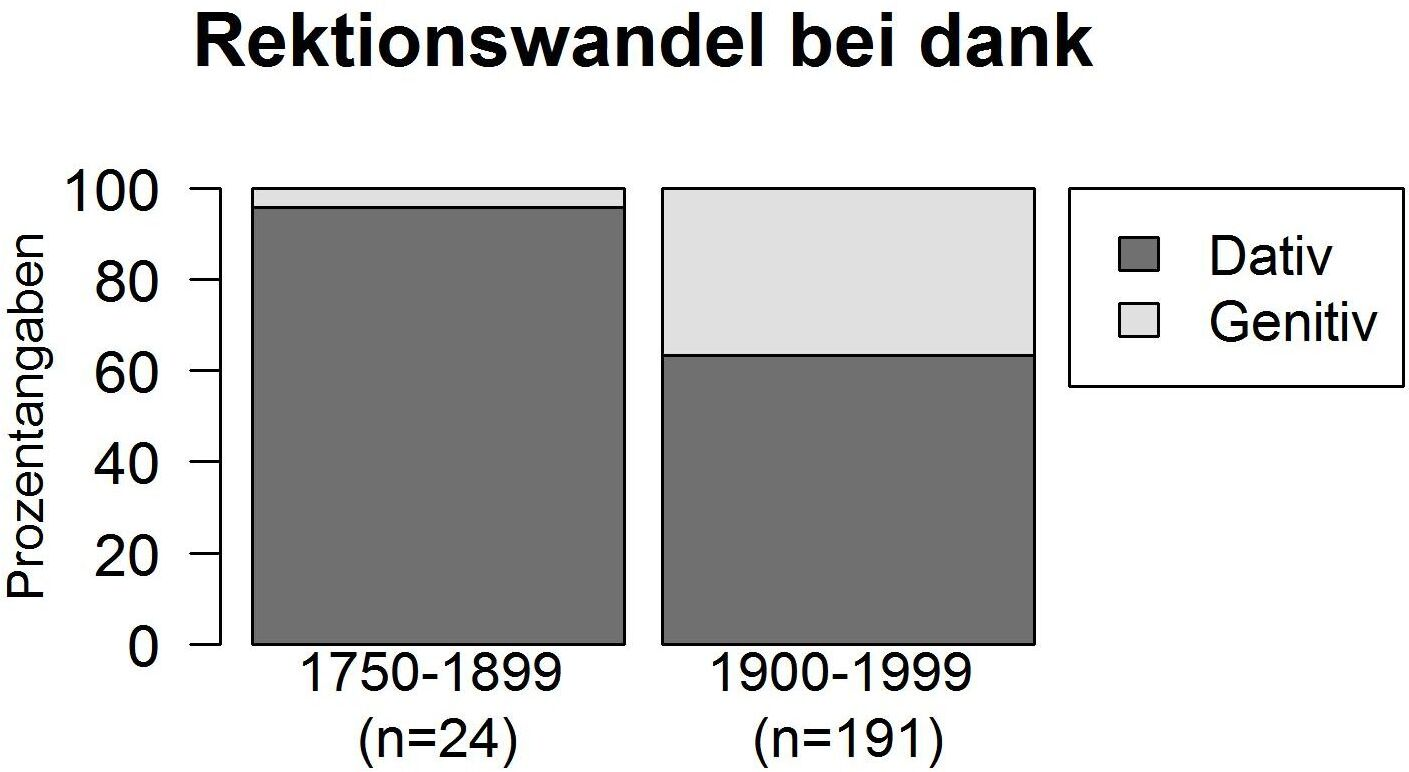
\includegraphics[scale=0.75]{Rektionswandeldank.jpg}
\caption{Kasusrektion von \object{dank} in Texten des DTA und des DWDS-Kernkorpus \citep[s.][]{Vieregge.2019}}
\label{pic:Rektionswandeldank}
\end{figure}

%Genitiv als Kasus denominaler Präpositionen
Diesen schnellen Übergang zur Genitivrektion erklärt \citet[25]{Agel1992} mit der Analogie zu semantisch ähnlichen Präpositionen wie \object{aufgrund} oder \object{infolge}. 
\citet[176]{DiMeola2004} weist jedoch darauf hin, dass Analogiebildungen keine hinreichende Erkl{\"a}rung bieten können, da sich für alle Fälle Gegenbeispiele finden lassen und unklar ist, warum einige Pr{\"a}positionen anf{\"a}llig sind, andere aber nicht. 
\citet[]{Eisenberg1979} sieht als Erklärung für die starke Tendenz von \dank{} zum Genitiv die Analogie zu anderen denominalen Präpositionen. 
Er versucht, eine klare Verteilung auszumachen, bei der die denominalen Pr{\"a}positionen zum Genitiv tendieren, die prim{\"a}ren Pr{\"a}positionen hingegen zum Dativ \citep[s.][519]{Eisenberg1979}. 
Allerdings lässt sich für die denominale Präposition \object{laut} im DTA und im DWDS-Kernkorpus beobachten, dass die Dativrektion vom 16. bis zum 20. Jahrhundert stetig ansteigt und schließlich ca. 90\,\% ausmacht \citep[s.][]{Vieregge.2019}. 

Ein weiterer Punkt spricht sowohl dagegen, dass die Tendenz zum Genitiv am nominalen Spenderlexem liegt, als auch dagegen, dass es sich dabei um die Differenzierung von einem solchen Spenderlexem handelt: 
Bei den ursprünglichen Genitivpräpositionen \wegen{} und \waehrend{} ist kein Wechsel zum Dativ erkennbar, wie bereits der kurze diachrone Ausblick in \citet[]{DiMeola2000} angedeutet hat. 
Die Korpusuntersuchung im DTA und DWDS-Kernkorpus zeigt, dass die Entwicklung hin zum Prototyp bei der deverbalen Präposition \waehrend{} deutlich gehemmt ist, wie in \autoref{pic:Rektionswandelwaehrend} zu sehen \citep[s.][]{Vieregge.2019}.

\begin{figure}
\centering
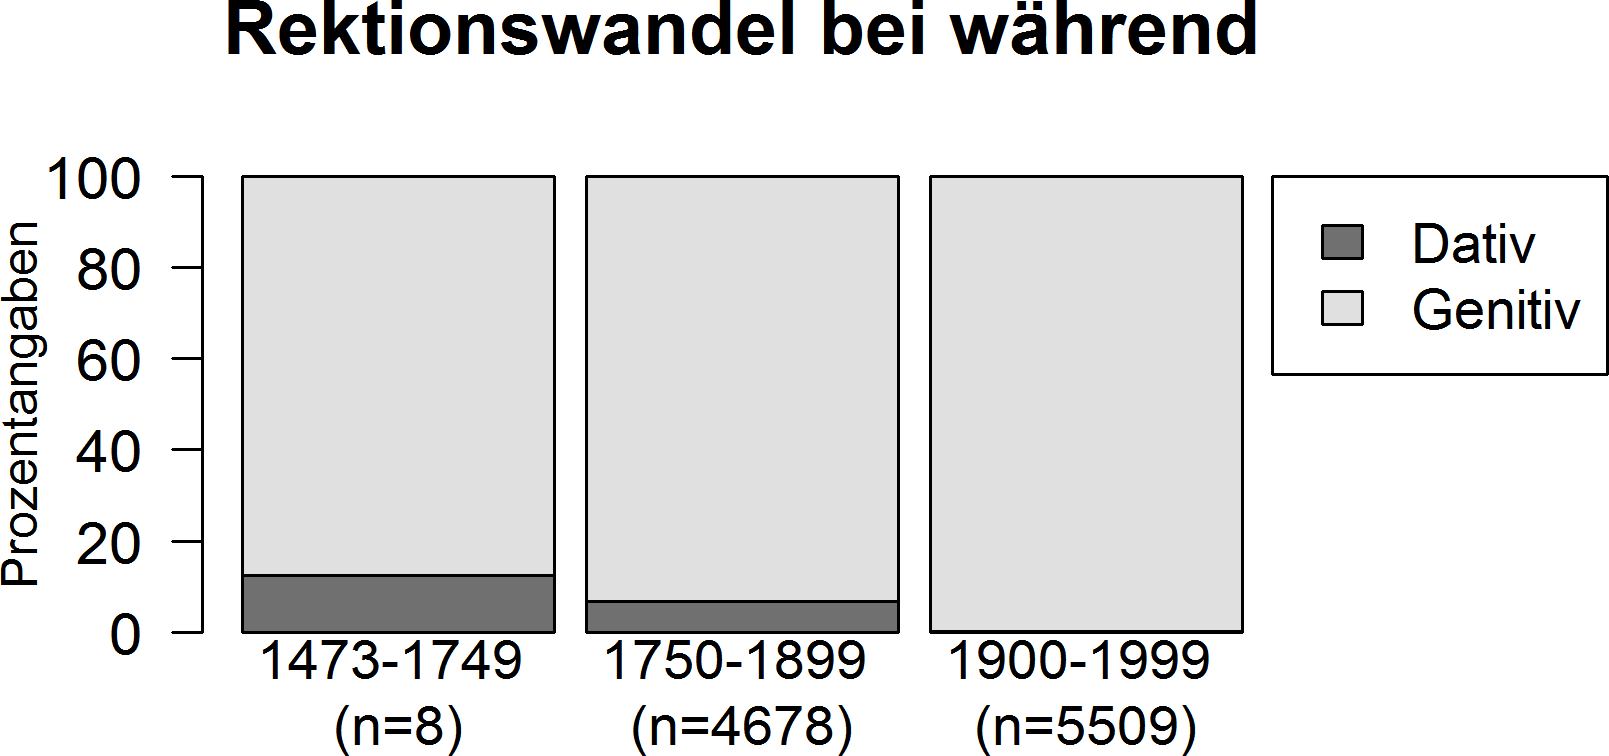
\includegraphics[scale=0.8]{Rektionswandelwaehrend.png}
\caption{Kasusrektion von \waehrend{} in Texten des DTA und des DWDS-Kernkorpus \citep[s.][]{Vieregge.2019}}
\label{pic:Rektionswandelwaehrend}
\end{figure}

\object{Während} wird im 18. Jahrhundert frequent. Von Beginn des Abdeckungszeitraums des DTA (1473) bis 1749 finden sich lediglich acht Belege für die Präposition, davon einer mit dem Dativ \citep[s.][]{Vieregge.2019}.
Zwischen 1750 und 1899 macht die Dativrektion 7\,\% der Belege aus. 
Im 20. Jahrhundert hingegen weisen von 5509 Belegen lediglich 14 eine Dativrektion auf, d.\,h., in 99,7\,\% der Fälle regiert die Präposition den Genitiv. 
Die Variation nimmt also deutlich zugunsten des Genitivs ab, eine Differenzierung von der Spenderstruktur erfolgt nicht. 

Ganz ähnliche Ergebnisse zur historischen Entwicklung der Rektion erhält \citet[]{Sato.2015}. 
Sie berücksichtigt die Präpositionen \wegen, \waehrend{} und \object{statt} in allen möglichen Stellungsvarianten mit Substantiven im Singular Maskulinum oder Neutrum in insgesamt 140 Gebrauchstexten von 1520 bis 1870 (je vier Texte pro Jahrzehnt) \citep[s.][30]{Sato.2015}. 
Die Studie zeigt eine Abnahme der Dativrektion bei \object{während} im 19. Jahrhundert \citep[s.][45--46]{Sato.2015}.
Für \wegen{}  stellt \citet[33]{Sato.2015} eine pl{\"o}tzliche Abnahme der Dativrektion ab 1800 fest: 
Der Dativ ist im 18. Jahrhundert signifikant h{\"a}ufiger als im 19. Jahrhundert, w{\"a}hrend f{\"u}r den Genitiv der umgekehrte Fall gilt~\citep[s.][34]{Sato.2015}.

%Produktionsexperiment Becker 2011
Dass sich die starke Tendenz zur Genitivrektion in der Gegenwartssprache fortsetzt, belegt ein Produktionsexperiment von \citet[]{Becker2011}. 
Sie legt 52 Studierenden zwei Lückentexte mit Sekundärpräpositionen vor, in denen jeweils die Flexionsendungen der Substantive und der Definitartikel in den Präpositionalphrasen ergänzt werden sollen \citep[s.][209]{Becker2011}. 
Die beiden Lückentexte unterscheiden sich laut \citet[209--210]{Becker2011} in der Formalität der gewählten Formulierungen. 
Da sich zwischen den beiden Lückentexten kaum Unterschiede ergaben, zeigt \autoref{table:Becker2011} eine Zusammenfassung aller Ergebnisse \citep[s.][210]{Becker2011}. 

\begin{table}
\centering
\begin{tabularx}{\textwidth}{Qcc}
\lsptoprule
                                                 & Anteil  & Anteil  \\
Laut kodifizierter Norm akzeptiert               & Genitivrektion & Dativrektion\\
\midrule
Nur Dativrektion (\object{gemäß, außer, gegenüber, entsprechend, entgegen})        & 65\,\%                    & 35\,\%                  \\
Dativ- und Genitivrektion (\object{einschließlich, während, laut, innerhalb, dank})  & 86\,\%                    & 14\,\%                  \\
Nur Genitivrektion  (\object{bezüglich,ungeachtet, hinsichtlich, längs, jenseits})  & 97\,\%                    & 3\,\%                   \\
\lspbottomrule
\end{tabularx}
\caption{Zusammenfassung der Ergebnisse aus \citet[210]{Becker2011}}
\label{table:Becker2011}
\end{table}

Die Ergebnisse lassen eine eindeutige Präferenz für den Genitiv erkennen: 
{\glqq}Es wurde selbst dann der Genitiv bevorzugt, wenn es sich um eine -- laut den Grammatiken eindeutige~-- Dativpr{\"a}position handelte{\grqq}~\citep[211]{Becker2011}. 
Bei der Präposition \object{gegenüber}, die im Korpus \citeauthor{DiMeola2000}s (\citeyear{DiMeola2000}) kaum schwankt, verwendeten in \citeauthor{Becker2011}s Experiment 54\,\% den Genitiv \citep[s.][211]{Becker2011}. 

Ebenfalls unerwartet vor dem Hintergrund der Differenzierungshypothese ist, dass sich in Korpora zumindest vereinzelt auch Belege für Primärpräpositionen mit dem Genitiv finden. 
\citet[259--260]{DiMeola2005b} etwa findet einige Belege für Primärpräpositionen mit Genitivrektion, bspw. für \object{seit} und \object{nach} \citep[s. auch][211]{DiMeola2009}. 
Auch \citeauthor{Vater.2009} (\citeyear[58]{Vater.2009} sowie \citeyear[220]{Vater.2015}) beobachtet den Genitiv bei der Prim{\"a}rpr{\"a}position \textit{seit}. 
Bei den Primärpräpositionen ist der Grammatikalisierungsprozess jedoch so weit vorangeschritten, dass das Differenzierungsprinzip nicht mehr greifen kann. 
Insgesamt scheint der Genitiv mit den meisten Präpositionen zumindest vereinzelt möglich zu sein. 
W{\"a}hrend bei den Beispielen, die \citeauthor{DiMeola2001} f{\"u}r ausschlie{\ss}liche Genitivpr{\"a}positionen anf{\"u}hrt, der Dativ tats{\"a}chlich nicht gebraucht wird (\textit{*diesseits dem Fluss, *zeit seinem Leben}), kommen etwa \object{fern} und \object{getreu}, die \citet[75--76]{DiMeola2001} als Beispiele f{\"u}r ausschlie{\ss}liche Dativpr{\"a}positionen anführt, im DWDS-Zeit-Korpus auch mit dem Genitiv vor. 
Für \object{getreu} finden sich lediglich vier, für \object{fern} jedoch ca. 70 Belege.
\citet[255]{DiMeola2005b} merkt außerdem an, dass von den urspr{\"u}nglichen Genitivpr{\"a}positionen bisher keine einzige vollst{\"a}ndig zum Dativ {\"u}bergegangen ist.
Der vollst{\"a}ndige {\"U}bergang von der Dativ- zur Genitivrektion l{\"a}sst sich hingegen laut \citeauthor{DiMeola2005b} (\citeyear[170]{DiMeola2004} sowie \citeyear[256]{DiMeola2005b}) bei \textit{trotz}, \textit{inmitten}, \textit{unfern }und \textit{unweit }beobachten. 

%\begin{quote}Der ungew{\"o}hnliche Vormarsch der Genitivrektion nach \textit{dank }zu Zeiten des allgemeinen Genitivr{\"u}ckgangs wird im Lichte des Determinativprinzips ebenfalls verst{\"a}ndlich. Da die Pr{\"a}postion auf eine Ellipse des Typs \textit{Dank [sei seinem Einflu{\ss} }zur{\"u}ckgeht (vgl. DU, S. 165), ist die urspr{\"u}ngliche Ausschlie{\ss}lichkeit der Dativrektion einleuchtend. Da jedoch die partiell synonymen Pr{\"a}positionen \textit{aufgrund, infolge, wegen }alle vom Determinativprinzip gesteuert werden, gesellt \textit{dank }sich langsam zu ihnen. \citep[25]{Agel1992}\end{quote}
%Analogie
%Zahlen aus dem DWDS.\footnote{Gesucht wurde mit Abfragen nach dem Muster "@dank @dem \#<2 \$p=NN".} \\
%\begin{table}
%\centering
%\label{RektionDWDS}
%\begin{tabular}{lcccc}
%\hline
 %                  & \multicolumn{2}{c}{1946-1981} & \multicolumn{2}{c}{1982-2016} \\
  %                 & Genitiv        & Dativ        & Genitiv        & Dativ        \\ \hline
%\textit{wegen}     & 99,0           & 1,0         & 99,5           & 0,5         \\
%\textit{während}   & 99,3           & 0,7         & 99,6           & 0,4         \\
%\textit{dank}      & 66,7           & 33,3         & 95,2           & 4,8         \\
%\textit{gegenüber} & 0           & 100         & 0,6           & 99,4        
%\\ \hline
%\end{tabular}
%\caption{Veränderung der Kasusrektion bei Sekundärpräpositionen}
%\end{table}
Die Daten zum Rektionswandel der Präpositionen zeigen deutlich, dass es eine starke Tendenz zum Genitiv gibt, während der Wechsel zur Dativrektion gebremst ist. 
Dies lässt sich mit dem Prototypisierungs- und dem Differenzierungsprinzip nicht ausreichend erklären. 
% Metapragmatik als Erklärungsfaktor
Offenbar ist die Entwicklung der Kasusrektion zusätzlich stark von der metapragmatischen Bewertung der Kasus beeinflusst. 
\citet[33--34]{Szczepaniak2014} etwa sieht die Aufladung mit sozialer Bedeutung und die Ideologie des Sprachverfalls als wesentliche Faktoren, die den Genitiv als Pr{\"a}positionalkasus f{\"o}rdern. 
\citet[36]{Lehmann1992} sprechen vom \glqq normativen Druck der Grammatiker\grqq{}, der den Genitiv begünstige. 
Ähnlich vermutet \citeauthor{Becker2011} als Grund für die starke Tendenz zum Genitiv in ihrem Produktionsexperiment, {\glqq}dass die Testpersonen mit dem Genitiv einen sozial markierten Sprachgebrauch verbinden und in der Testsituation ein entsprechendes Erwartungsmuster erf{\"u}llen wollten{\grqq}~\citep[211]{Becker2011}. 
\citet[218]{DiMeola2000} selbst misst der metapragmatischen Bewertung keine große Bedeutung bei. 
Er diskutiert ihren Einfluss unter dem Punkt {\glqq}Rolle der Standardisierung{\grqq} und kommt zu dem Schluss, dass hier {\glqq}Ursache und Wirkung verwechselt werden. Standardisierung hat n{\"a}mlich in erster Linie ratifizierenden, nicht propositiv-pr{\"a}skriptiven Charakter{\grqq} \citep[216]{DiMeola2000}. 
Dabei scheint er jedoch die komplexen Zusammenhänge zwischen Aussagen in Kodizes, Sprachideologien und dem Sprachgebrauch zu übersehen (\autoref{sec:MetapragmatikVariationWandel}). 
Auf diese wird im folgenden Abschnitt eingegangen, der sich der Indexikalität der Präpositionalkasus als wesentlichem Faktor für die Variation und den Wandel der Präpositionen widmet. 
\section{Die Indexikalität der Rektionskasus} \label{sec:IndexikalitaetRektionskasus}
In den folgenden Abschnitten werden bisherige Studien vorgestellt, die auf die Registrierung und die Indexikalität der Rektionskasus hindeuten. 
Dabei soll zunächst auf Korpusstudien eingegangen werden, die einen Einblick in die Registrierung der Varianten geben (\autoref{sec:KorpusstudienRektion}). 
Anschließend wird in \autoref{sec:IndexikalitaetRektionskasushistorisch} dargestellt, inwiefern historische Grammatiken und sprachpflegerische Schriften zur Registrierung beigetragen haben.  
\autoref{sec:IndexikalitaetRektionskasusheute} geht auf Untersuchungen ein, die Hinweise darauf liefern, welche soziale Bedeutung die Präpositionalkasus heute für Sprecher:innen des Deutschen haben. 
\subsection{Anhaltspunkte aus korpusbasierten Studien}
\label{sec:KorpusstudienRektion}
%Im von \citeauthor{Scott.2014} durchsuchten Zeitungskorpus GerManC, das Texte von 1650 bis 1800 enth{\"a}lt und insgesamt 100000 W{\"o}rter umfasst, kommt \textit{wegen} 68mal mit dem Genitiv und sechsmal mit dem Dativ vor, au{\ss}erdem zweimal mit dem Akkusativ. \textit{W{\"a}hrend }findet sich lediglich viermal, davon dreimal mit dem Genitiv~\citep[s.][243]{Scott.2014}. \\
Zwar zielen die bisherigen korpuslinguistischen Studien nicht darauf ab, explizite metapragmatische Äußerungen zur Registrierung der Rektionsvarianten zu erfassen, jedoch bieten Erkenntnisse zur Verteilung in Korpora implizite Hinweise darauf, welchen Registern eine Variante zugeordnet wird. 
Korpusstudien sind daher insbesondere für die \textit{presupposition}, also die Angemessenheit einer Variante im Kontext, aufschlussreich (\autoref{sec:Indexikalitaet}). 

\citet[]{DiMeola2000} untersucht in seiner Korpusstudie, wie sich die Rektionsvarianten auf verschiedene Textsorten verteilen. 
Dazu unterscheidet er zwischen folgenden fünf Textsorten: Pressesprache (Ausgaben der FAZ), Fachtexte (an ein Fachpublikum gerichtete rechts- und wirtschaftswissenschaftliche Texte), Sachprosa (Ratgeber und Reiseführer), Belletristik (Werke von 20 Schriftsteller:innen) und Unterhaltungsliteratur (von \citeauthor{DiMeola2000} näher angegeben als Kriminalromane und Frauenliteratur).\footnote{Unter Frauenliteratur fasst \citet{DiMeola2000} elf (Liebes-)Romane aus dem Unterhaltungsbereich, alle von weiblichen Verfasserinnen. Zu den Titeln gehören bspw. Dünnebier, Anna, \textit{Der Quotenmann} oder Luginger, Karin \textit{Männer fallen nicht vom Himmel}.} 
Die Genitivrektion bei ursprünglichen Dativpräpositionen kommt häufiger in nicht-fiktionalen Texten vor. 
So findet sich bspw. bei \dank{} in allen Textsorten häufiger die Genitivrektion, in Fach- und Pressetexten kommt sie aber ausschließlich vor \citep[s.][212]{DiMeola2000}. 
Die Dativrektion bei \textit{wegen }und \textit{w{\"a}hrend }kommt im Korpus \citeauthor{DiMeola2000}s hingegen insbesondere in Belletristik und Unterhaltungsliteratur vor \citep[s.][210]{DiMeola2000}. 
Der historisch neuere Dativ bei \textit{wegen }kommt 112-mal von 147-mal in fiktionalen Texten vor. 
Bei \waehrend{} kommt die Dativrektion in \citeauthor{DiMeola2000}s Korpus insgesamt lediglich zehnmal vor, davon achtmal in fiktionalen Texten. 
Hier zeigt sich also eine Ausdifferenzierung der Kasus nach Textsorten:~W{\"a}hrend die nicht-fiktionalen Texte zum Genitiv tendieren, wird in den fiktionalen Texten der Dativ bevorzugt.
Diese Textsortenaffinität kann auf die unterschiedliche Registrierung der Rektionsvarianten hindeuten. 
Eine solch starre Textsorteneinteilung wie sie bei \citet{DiMeola2000} und auch in vielen anderen Korpusuntersuchungen vorgenommen wird, ist allerdings problematisch, da bspw. nicht ersichtlich ist, in welchen Kontexten die Rektionsvarianten tatsächlich verwendet werden und welche Wirkung sie dort haben. 

Während die Texte im Korpus \citeauthor{DiMeola2000}s alle zur lektorierten Schriftlichkeit gehören, untersucht \citet[]{Elspa2005} private Briefe von Emigrant:innen aus dem 19. Jahrhundert. 
Er betrachtet unter anderem die Rektion der Präposition \wegen{} und findet 71 Belege, die eindeutig einem Kasus zugeordnet werden k{\"o}nnen. 
Davon weisen lediglich acht eine Genitivrektion auf, 45-mal wird der Dativ verwendet und 18-mal der Akkusativ~\citep[s.][321]{Elspa2005}.\footnote{Die Akkusativrektion erklärt \citet[]{Elspa2005} mit dem Einfluss von Dialekten, in denen Akkusativ und Dativ häufig zusammenfallen.}
Insbesondere unge{\"u}bte Schreiber:innen verwenden den Dativ oder den Akkusativ, in den Briefen routinierter Schreiber:innen hingegen findet sich in vier von sechs Fällen der Genitiv \citep[s.][321--323]{Elspa2005}. 
Ein diachroner Vergleich zeigt, dass der Dativ in den Briefen vom 17. bis zum 19. Jahrhundert h{\"a}ufiger wird, sodass im 19. Jahrhundert in der informellen Schriftlichkeit die Dativrektion {\"u}berwiegt~\citep[s.][411]{Elspa.2015}. 
In Texten aus dem Zeitungskorpus des GerManC und dem Kaiserreich-Corpus (KuK-Corpus), die zusammen den Zeitraum 1650 bis 1918 abdecken, wird \wegen{} hingegen {\"u}berwiegend mit dem Genitiv gebraucht~\citep[s.][410]{Elspa.2015}. 
\citeauthor{Elspa2005} schlie{\ss}t aus der Verteilung der Rektion, \begin{quote}dass der Gebrauch von Pr{\"a}positionen, die den Genitiv regieren sollen, im 19. Jahrhundert nicht in der Alltagssprache verwurzelt, sondern ein Merkmal gebildeter Schreibender war.~\citep[321]{Elspa2005}\end{quote}
\citet[]{Sato.2015} nimmt in einer stärker qualitativ ausgerichteten Untersuchung die Kasuswahl nach \wegen{}, \waehrend{} und \object{statt} in verschiedenen Schriften Beethovens in den Blick.  Sie betrachtet zum einen die Konversationshefte, durch die der am Ende seines Lebens mehr und mehr gehörlose Beethoven mit Angehörigen und Bekannten kommunizierte, zum anderen aber auch Briefe und eine theoretische Schrift. 
Zwar zeigt sich eine eindeutige Verteilung, da in der theoretischen Abhandlung ausschließlich der Genitiv gebraucht wird, in den sehr informellen Konversationsheften dagegen fast ausschließlich der Dativ \citep[s.][27]{Sato.2015}. 
Die Belegzahlen sind allerdings sehr gering (zwischen fünf und 130 Belege pro Textsorte) und es handelt sich um einen einzigen Schreiber. 
Da zwischen einzelnen Schreiber:innen immer individuelle Unterschiede zu erwarten sind, ist dies für eine variationslinguistische Untersuchung nicht optimal. 
Interessant ist aber der Blick auf die Kasuswahl mit verschiedenen Kommunikationspartner:innen. 
Beethovens Neffe Karl wählt in der Kommunikation mit seinem Onkel, zu dem er kein gutes Verhältnis hatte, häufiger den Genitiv als mit anderen Kommunikationspartner:innen, was \citet[s.][29]{Sato.2015} als Mittel deutet, Distanz zu evozieren. 
% Änderung Anfang 
In \citet{Sato.2022} werden neben Beethovens Briefen und Konversationsheften private Briefe von Haydn, Bach, Goethe und der Familie Mozart berücksichtigt.
Die Auswertung der Briefe von Mitgliedern der Familie Mozart zeigt bspw., dass die Genitivrektion bei \wegen{} in Briefen an Familienangehörige signifikant seltener ist als in Briefen an Personen, die nicht zur Familie gehören \citep[s.][96--97]{Sato.2022}. 

In einer Untersuchung von \wegen{} in 39 zwischen 1750 und 1850 erschienenen Dramen zeigt \citet[]{Sato.2016} außerdem, dass Dramenfiguren aus oberen Schichten bei dieser Präposition h{\"a}ufiger der Genitiv in den Mund gelegt wird, Figuren aus unteren Schichten dagegen der Dativ~\citep[s.][409]{Sato.2016}: 
54 von 59 Vorkommen von \wegen{} mit Genitivrektion lassen sich Figuren der oberen Schichten zuordnen, 17 von 20 Vorkommen mit Dativrektion hingegen Figuren aus unteren Schichten.

% gesprochene Sprache 
Die Kasuswahl in gesprochener Sprache untersucht \citet[]{Petig1997}. 
Er wertet zwei Korpora (das Pfeffer-Korpus von 1961 und das Jones-Korpus von 1992) mit insgesamt 800 ca. zehnminütigen Interviews zu verschiedenen Themen aus~\citep[s.][36]{Petig1997}.\footnote{Zu den Themen schreiben \citet[17]{Pfeffer.1984}, dass zwar zunächst jeweils eines von 25 zuvor bestimmten Themen, wie etwa Wetter, Schule und Erziehung oder Freizeit, vorgegeben war, die Gesprächspartner:innen von diesem aber häufig abwichen, wodurch \glqq die Natürlichkeit und Ungezwungenheit erhöht\grqq{} worden sei.} 
Unter den Sprecher:innen des Korpus finden sich je ca. 200 Frauen und Männer aller Alters- und Bildungsgruppen aus verschiedenen Regionen in Deutschland, {\"O}sterreich und der Schweiz \citep[s.][17]{Pfeffer.1984}. 
\citeauthor{Petig1997} betrachtet die Präpositionen \object{während}, \object{wegen}, \object{(an)statt} und \object{trotz} mit Maskulina oder Neutra im Singular und Plural. 
\object{(An)statt} und \object{trotz} kommen nur selten vor, \wegen{} und \waehrend{} sind deutlich frequenter. 
Sie treten in den Interviews allerdings beide nur sehr selten mit dem Dativ auf~\citep[s.][37]{Petig1997}: 
Lediglich zwischen 4\,\% (\waehrend{} im Pfeffer-Korpus) und 11\,\% (\wegen{} im Jones-Korpus) der Belege entfallen auf die Dativrektion \citep[s.][37]{Petig1997}. 
Die wenigen Belege mit der Dativrektion finden sich insbesondere in s{\"u}ddeutschen Dialekten~\citep[s.][38]{Petig1997}. 
Dieser Befund deutet scheinbar darauf hin, dass die Genitivrektion in der gesprochenen Sprache die deutlich häufigere Variante ist. 
Ob dies jedoch auf natürliche Interaktionssituationen übertragbar ist, ist fraglich. 
\citet[37]{Petig1997} selbst weist darauf hin, \glqq that people may speak more formally in an interview situation when they know they are being recorded.\grqq{}

Die regionale Verteilung der Rektionsvarianten betrachtet auch \citet{Elter2005}. 
Anhand einer Untersuchung der Pr{\"a}positionen \wegen, \waehrend, \dank, \object{trotz} und \object{statt} mit Definitartikel im Maskulinum oder Neutrum in Zeitungen aus Deutschland, Österreich und der Schweiz zeigt sie, dass es in der Zeitungssprache insgesamt wenige Belege mit Dativ gibt \citep[s.][128]{Elter2005}. 
\textit{Wegen} regiert in 0,8\,\% der Belege den Dativ, \waehrend{} in 0,3\,\%, \dank{} in 7\,\% \citep[s.][128]{Elter2005}. 
Dabei lassen sich regionale Unterschiede beobachten. 
So regiert \dank{} in schweizerdeutschen Zeitungen weitaus h{\"a}ufiger den Dativ~\citep[s.][134]{Elter2005}. 
Bei \waehrend{} entfallen fast alle Belege für die Dativrektion auf die Schweiz, bei \wegen{} ist die Verteilung hingegen weniger deutlich \citep[s.][130--131]{Elter2005}.
Die Dativrektion könnte von Sprachbenutzer:innen potenziell also als indexikalischer Verweis auf schweizerdeutschen Sprachgebrauch gedeutet werden. 
In \citeauthor{Elter2005}s Untersuchung deutet sich außerdem an, dass der Dativ als Pr{\"a}positionalkasus bei Sekund{\"a}rpr{\"a}positionen offenbar verwendet wird, um Umgangssprache bzw. m{\"u}ndlichen Sprachgebrauch zu evozieren, wie etwa in diesem Beispiel \citep[s.][128--129]{Elter2005}:
\begin{exe}
\ex \ExampleFont{Die anderen Bandmitglieder haben {\glq}Number Nine{\grq} wegen ihres fortgeschrittenen Alters verlassen... {\glq}Wir spielen, was die Leute h{\"o}ren wollen{\grq}, erkl{\"a}rt Frank das Song-Repertoire, setzt allerdings gleich hinzu:~{\glq}Aber nicht alles! Die  {\glq}B{\"o}hsen Onkelz{\grq} haben wir nie performed, wegen dem Nazi-Image.{\grq}} (Nordbayrische Nachrichten, 14.12.2002, Beispiel aus \citealp[129]{Elter2005})
\end{exe}
Gerade für \wegen{} stellt \citet[128]{Elter2005} fest, dass die Dativrektion häufig in wörtlichen Zitaten auftritt. 
Diese Verteilung spricht für eine Registrierung des Dativs als mündlichkeitsnah.

Die Registrierung des Dativs als informell und des Genitivs als formell wird durch verschiedene weitere Faktoren gestützt. 
Ein Faktor besteht darin, dass es in den Dialekten des Deutschen so gut wie keinen Genitiv gibt (\cites[s.][437]{Shrier.1965}[250]{Scott.2014}). Lediglich in einigen wenigen Dialekten werden noch Genitive gebraucht, bspw. in der schweizer Region Wallis \citep[s.][1243]{Ko.1983}.\footnote{\citet[339]{Scott.2014} weist darauf hin, dass empirische Untersuchungen dazu, welche Formen und Funktionen des Genitivs in Dialekten des Deutschen überhaupt vorhanden sind, noch ausstehen. Für das Luxemburgische zeigt \citet{Dohmer.2018}, dass Genitive vorhanden, aber nur eingeschränkt produktiv sind. \citet{Hoge.2018} argumentiert, dass das Jiddische einen possessiven Genitiv aufweise.} 
Da Dialekte in der Vorstellung der Sprachbenutzer:innen für eher informelle, private kommunikative Praktiken genutzt werden, begünstigt dies die Wahrnehmung des Dativs als informell~\citep[s.][221--222]{Maitz2015}. 
Hinzu kommt, dass der Genitiv nicht nur als Präpositionalkasus, sondern auch als Attribut- und Objektkasus eher in formellen Registern zu verorten ist, wie \citet[252]{Scott.2014} anhand eines Vergleichs von Spiegel-Artikeln mit dem Dortmunder Chat-Korpus sowie gesprochener Sprache aus dem Wende-Korpus zeigt. 
Als Grund daf{\"u}r, dass der Genitiv in informellen Registern seltener ist, sieht \citet[s.][276]{Scott.2014} jedoch nicht eine Vermeidung des Kasus, sondern vielmehr, dass Strukturen, in denen ein Genitiv als Variante m{\"o}glich w{\"a}re, insgesamt seltener sind: 
\glqq the connection of two noun phrases in a broadly possessive relationship and the use of genitive-assigning prepositions is simply rare in informal language use\grqq{}~\citep[276]{Scott.2014}.

%Registrierung Sekundärpräpositionen
Ein weiterer Faktor, der die Registrierung der Rektionskasus stützt, ist die Registrierung der Sekundärpräpositionen selbst als formell und schriftsprachlich. 
Zwar kommen sie auch in gesprochener Sprache vor, wie eine Untersuchung von \citet[]{Mikosch1987} zeigt, die auf Transkriptionen süddeutscher dialektaler Gesprächsdaten aus den 50er Jahren basiert. 
Bis auf \wegen{} sind sie hier jedoch nur selten vertreten; \dank{} findet sich in den Daten \citeauthor{Mikosch1987}s (\citeyear[125]{Mikosch1987}) bspw. überhaupt nicht.
\citet[48]{Bene.1975} sch{\"a}tzt, dass die sehr wenig prototypischen Pr{\"a}positionen vor allem in Wissenschafts- und Sachregistern angesiedelt sind. 

Im Rahmen der oben bereits beschriebenen Korpusuntersuchung im DWDS-Kernkorpus \citep[s.][]{Vieregge.2019} wurde die Verteilung von \waehrend, \dank, \object{laut} und \object{entsprechend} auf die dort angelegten Textsorten \glqq Zeitung\grqq, \glqq Wissenschaftssprache\grqq, \glqq Gebrauchsliteratur\grqq{} und \glqq Belletristik\grqq{} untersucht. 
\autoref{pic:TextsortenDWDS} zeigt die Verteilung der Treffer für die gesuchten Präpositionen plus \object{dem} oder \object{des} im Vergleich zur Verteilung aller Tokens im Korpus.

\begin{figure}
\centering
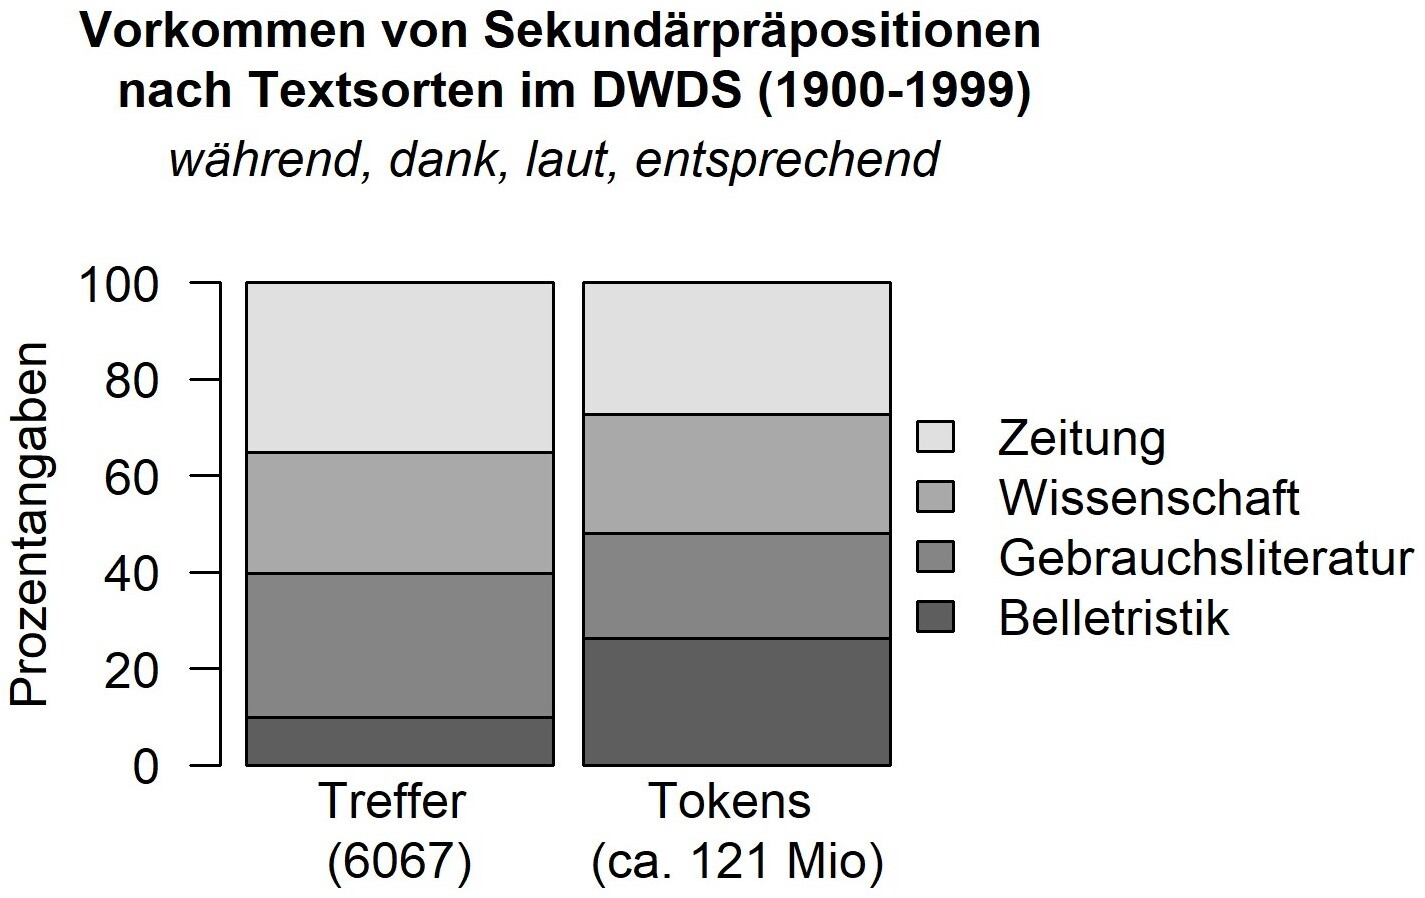
\includegraphics[scale=0.8]{TextsortenDWDS.jpg}
\caption{Textsortenverteilung von \waehrend, \dank, \object{laut} und \object{entsprechend} \citep[s.][]{Vieregge.2019}}
\label{pic:TextsortenDWDS}
\end{figure}

Bis auf den Bereich Wissenschaftssprache lässt sich keine dieser Textsorten pauschal als formelles oder informelles Register bezeichnen. 
Dennoch ist es interessant, mit welchen Textsorten der Gebrauch dieser Sekundärpräpositionen verknüpft ist. 
Wie man sehen kann, ist die Verteilung der untersuchten Sekundärpräpositionen anders als die aller Tokens im Korpus. 
Die gesuchten Konstruktionen zeigen eine leichte Affinität zur Zeitungssprache sowie zu Gebrauchstexten. 
In der Belletristik kommen die Sekundärpräpositionen hingegen seltener vor, in der Wissenschaftssprache zeigt sich kein Unterschied zur Verteilung aller Tokens \citep[s.][]{Vieregge.2019}. 
Ein Chi-Quadrat-Test zeigt, dass der Unterschied zwischen der Textsortenverteilung der gesuchten Sekundärpräpositionen und der aller Tokens signifikant ist, aber nur eine geringe Effektstärke aufweist ($\chi^2=30{,}7$, $p<0{,}001$, $\text{Cramers V}=0{,}071$).
In der Tendenz kommen Sekundärpräpositionen also vor allem in informationsorientierten Texten vor.

\citet[176--184]{DiMeola2000} überprüft bei seiner Korpusuntersuchung die Textsortenverteilung für einzelne Präpositionen. 
Für \waehrend{} stellt er fest, dass die Präposition am häufigsten in Sachtexten vertreten ist.
\object{Wegen} und \dank{} kommen hingegen insbesondere in Pressetexten vor und \gegenueber{} in fachsprachlichen Texten. 
Insgesamt kommt \citet[184]{DiMeola2000} zu dem Schluss, dass Sekundärpräpositionen typisch für fachsprachliche Texte seien, während Primärpräpositionen keine textsortenspezifische Verteilung zeigten. 
Die Genitivrektion wird also auch deswegen als formell registriert, weil die Sekund{\"a}rpr{\"a}positionen, von denen die meisten den Genitiv regieren, vor allem in formellen Registern vorkommen~\citep[s.][209]{Becker2011}. 

Zusammenfassend lässt sich festhalten, dass korpusbasierte Studien bereits einige Anhaltspunkte zur Registrierung der Rektionskasus von Sekundärpräpositionen bieten. 
Bei \citet[]{DiMeola2000} zeigt sich, dass die Dativrektion insgesamt selten ist und dabei in fiktionalen Texten häufiger vorkommt als in nicht-fiktionalen. 
In der privaten Schriftlichkeit des 19. Jahrhunderts nutzen geübte Schreiber:innen die Genitivrektion eher als ungeübte Schreiber:innen \citep[s.][]{Elspa.2005}. 
Dies deutet auf eine frühe Assoziation des Kasus mit Bildung und dadurch auch mit der Standardsprache als Varietät der Bildungsschicht hin. 
In historischen Zeitungstexten findet sich vorwiegend die Genitivrektion \citep[s.][]{Elspa.2015}. 
Während der Genitiv also verstärkt in Registern des öffentlichen Sprachgebrauchs auftritt, lässt sich der Dativ im Privaten verorten. 
Dies bestätigen qualitative Untersuchungen von \citeauthor{Sato.2015} (\citeyear{Sato.2015} und \citeyear{Sato.2016}) zum Sprachgebrauch Beethovens und zu Dramentexten. 
In den von \citet{Petig1997} untersuchten gesprochensprachlichen Korpora finden sich erstaunlich wenige Fälle von Dativrektion.
Sollte dies ein Effekt sozialer Erwünschtheit sein, so wäre auch dies ein Hinweis auf die Indexikalitäten der Kasus: 
\citet[37]{Petig1997} vermutet, die Interviewpartner:innen gingen davon aus, mit der Verwendung der Genitivrektion einen besseren Eindruck zu hinterlassen.
Ob es für diese Vermutung konkrete Anhaltspunkte in den Interviews gibt, bleibt allerdings unklar. 
Auf eine mögliche Registrierung als regionalspezifisch deutet die Untersuchung zu Zeitungstexten von \citet{Elter2005} hin, in der die Dativrektion v.\,a. in der Schweiz vorkommt. 
\subsection{Registrierung durch Grammatiken und sprachpflegerische Schriften} \label{sec:IndexikalitaetRektionskasushistorisch}
Für die Registrierung als sprachideologischen Prozess ist nicht nur die Verteilung in Korpora relevant, sondern insbesondere der metapragmatische Diskurs. 
Dieser wird im Folgenden zunächst anhand von Analysen historischer Grammatiken und sprachpflegerischer Schriften beleuchtet. 

% Historische Grammatiken 
\begin{sloppypar}
\citet{Davies2006} untersuchen Sprachurteile in Grammatiken und sprachpflegerischen Schriften von 1600 bis 2005.
Für \wegen{} stellen sie fest, dass die Präposition im 17. Jahrhundert zwar sowohl als Dativ- als auch als Genitivpr{\"a}position beschrieben wird, die Toleranz der Grammatiker von da an aber abnimmt~\citep[s.][202]{Davies2006}.
Die erste Erwähnung von \wegen{} findet sich 1641 in Gueintz' Sprachlehre, hier wird als Rektionskasus nur der Dativ genannt~\citep[s.][209]{Davies2006}. 
Die erste Stigmatisierung der Dativrektion findet sich dann bereits bei \citet[245]{Heynatz.1777}: 
\glqq Es ist unrichtig, wenn man \object{anstatt}, \object{längst}, \object{während} und \wegen{} anstatt des Genitivs mit dem Dativ setzt.\grqq{}
Noch negativer äußert sich \citet[]{Matthias.1929} in seinem erstmals 1892 erschienenen Werk \glqq Sprachleben und Sprachschäden\grqq:
\end{sloppypar}

\begin{quote} Durchaus gebührt \object{ohne} der vierte Fall: \object{ohne dich, ohne das Kind}, und \wegen{} der zweite: \object{wegen des Vergehens} oder \object{des Vergehens wegen}. […] [D]agegen hüte man sich, die volksmäßige Verunstaltung: \object{mit jemand von wegen einem Vorkommnisse reden müssen} u.\,ä. nachzuahmen. \citep[141]{Matthias.1929} \end{quote}
Der Dativ wird also explizit abgewertet und mit Volkstümlichkeit in Verbindung gebracht. 
Dass die Dativrektion in manchen Fällen auch in der formellen Schriftlichkeit akzeptiert wird (etwa bei artikellosen Substantiven im Plural wie in \object{wegen Ästen}), findet bis in die 1980er Jahre kaum Erwähnung und wird somit ausgeblendet \citep[s.][205, 209]{Davies2006}. 
Die Studie von \citet[]{Davies2006} zeigt, dass die Registrierung des Genitivs als Prestigekasus und die Stigmatisierung des Dativs Prozesse sind, die sich seit dem 18. Jahrhundert bis heute fortsetzen. 
Zusammenfassend konstatieren \citeauthor{Davies2006}:\begin{quote}The genitive case is considered to be a proud and important case of German grammar and any developments in favour of other cases are frowned upon and should be fought. \citep[209]{Davies2006}\end{quote}
% Grammatiken heute
Heute wird sowohl in der Sprachwissenschaft als auch von Grammatiken und im laienlinguistischen Diskurs immer darauf hingewiesen, die Variation zwischen Genitiv- und Dativrektion orientiere sich im Wesentlichen am Register (\cites[s. etwa][172]{Barbour1998}[135]{Elter2005}[182]{Eisenberg.2013}).  
Der \citeauthor{Duden2022} gibt an: 
\begin{quote}Einige genitivregierende Präpositionen erlauben auch den Dativ (z. B. (an)statt, fern, zuzüglich). Die Dativrektion ist vor allem in gesprochener Sprache häufig, aber auch im geschriebenen Deutsch zu finden, allerdings in sehr unterschiedlicher Frequenz.~\citep[{\S}1450]{Duden2022}\end{quote}
%\begin{quote}Prinzipiell hat man bei der Kasuswahl Freiheit, sieht man von Stilunterschieden ab. Der Genitiv gilt als eher schriftsprachlich und stilistisch h{\"o}her stehend.~\citep[{\S}910]{Duden2016}\end{quote}
Ältere Dudenausgaben allerdings führen \wegen{} ausschlie{\ss}lich unter dem Eintrag zu den Genitivpr{\"a}positionen auf \citep[s.][208]{Davies2006}. 
\citet[358]{Helbig.2017} bezeichnen die Dativrektion bei \textit{wegen }und \textit{w{\"a}hrend }sowie bei anderen urspr{\"u}nglichen Genitivpr{\"a}positionen als \glqq umgangssprachlich\grqq, wird sie nicht als Ersatz f{\"u}r einen nicht erkennbaren Genitiv im Plural gebraucht. 
Die Genitivrektion bei urspr{\"u}nglichen Dativpr{\"a}positionen wie \textit{dank }oder \textit{zufolge }hingegen wird nicht als umgangssprachlich bezeichnet, sondern lediglich als Variante neben der Dativrektion aufgef{\"u}hrt~\citep[s.][358]{Helbig.2017}. 
Damit wird der Wandel zur Dativrektion implizit gegenüber dem Wandel zur Genitivrektion abgewertet. 

%Bastian Sick
Besondere Prominenz haben die sprachpflegerischen Kolumnensammlungen Bastian \citeauthor{Sick2006}s erhalten, deren Titel \textit{Der Dativ ist dem Genitiv sein Tod} zu einem Topos im Diskurs um den Genitiv geworden ist. 
Zu \wegen{} liest man dort etwa: 
\begin{quote} Welch wohlklingende Wortwahl: wegen des Winterwetters! Und dagegen nun der schnöde Dativ: wegen dem Winterwetter. Was klingt besser? \citep[101]{Sick2006} \end{quote}
Die Funktion der bewusst unterhaltsam geschriebenen Texte besteht insbesondere in der Abgrenzung gegenüber Gruppen, denen der Gebrauch der Dativrektion und anderer stigmatisierter sprachlicher Formen zugeschrieben wird.  
\citeauthor{Sick2006} und seinem Wirken wird eine wichtige Rolle bei der Verbreitung der Ideologie vom Aussterben des Genitivs zugesprochen: 
\begin{quote}Although the idea that the genitive case is in mortal danger (particularly as a result of encroachment from the dative)~is not new, Sick has certainly contributed greatly to the perception of a genitive under threat, and his title has entered the popular consciousness.~\citep[24]{Scott.2014}\end{quote}
\citet[323]{Langer.} verweist daneben aber auch auf Medien wie Die Zeit, den Spiegel und die S{\"u}ddeutsche Zeitung sowie den Sprachpfleger Wolf Schneider, die in Artikeln den Verlust des Genitivs und damit einhergehend eine {\glqq}Verarmung geistiger Ausdruckskraft{\grqq} beklagten. 
\citet[9]{Krause2012b} stellt die aus ihrer Sicht hyperkorrekte Verwendung des Genitivs in einen direkten Zusammenhang mit popul{\"a}rwissenschaftlichen Werken wie denen \citeauthor{Sick2006}s. 
In einer Untersuchung des Rektionsverhaltens von \object{entlang} kann sie allerdings keinen zeitlichen Zusammenhang zwischen einer Zunahme der Genitivrektion und dem Erscheinen von \citeauthor{Sick2006}s Schriften feststellen \citep[s.][347]{Krause2012a}. 
Dennoch betrachtet sie, ähnlich wie \citet[211]{Becker2011}, die Indexikalität der Genitivrektion als Grund für ihre hohe Frequenz: 
Als Motivation, den Genitiv zu w{\"a}hlen, sieht \citet[19]{Krause2012b}, {\glqq}dass im Zweifelsfall der Genitiv das Elegantere, Rettenswerte, Vornehmere ist{\grqq}. 

% Stigmatisierung hyperkorrekter Genitiv
\begin{sloppypar}
\citeauthor[]{Scott.2014} weist darauf hin, dass auch der Gebrauch des Genitivs mit urspr{\"u}nglichen Dativpr{\"a}positionen bereits seit Jahrhunderten stigmatisiert wird: \glqq Frequently, this use of the genitive is objected to by those who otherwise decry the replacement of the genitive\grqq{} \citep[303]{Scott.2014}.
Dies lässt sich z.\,T. auch noch in neueren Grammatiken beobachten. 
\citet[374]{Jung1980} schreibt zu \textit{dank }:\textit{~}{\glqq}\textit{dank }fordert den Dativ (der Genitiv ist weniger gut){\grqq}.
Ebenso macht \citeauthor{Sick2006} sich über den \glqq hyperkorrekten\grqq{} Gebrauch des Genitivs bei Präpositionen wie \object{trotz} lustig \citep[s.][210]{Davies2006}. 
F{\"u}r \dank{} mit Genitivrektion l{\"a}sst sich in den Grammatiken allerdings eine sehr rasche Verbreitung im Vergleich zu \wegen{} mit Dativ feststellen~\citep[s.][257]{Baumann2014}. 
Auch dies kommt einer impliziten Bevorzugung des Genitivs gleich. 
\end{sloppypar}

% Baumann/Dabóczi, Schulen
Neben Grammatiken und sprachpflegerischen Schriften zählt auch die Schule zu den Sprachautoritäten, die den Diskurs um die Rektionskasus prägen. 
\citet{Baumann2014} führen eine Umfrage unter angehenden und praktizierenden Lehrer:innen durch, in der sie unter anderem nach der Akzeptabilität von \wegen{} und \dank{} mit der Dativrektion in Schülertexten fragen. 
Obwohl der Duden zum Zeitpunkt der Befragung jeweils beide Rektionsvarianten als korrekt angibt, wird die Dativrektion bei beiden Präpositionen nur von ca. der Hälfte der 92 Befragten akzeptiert \citep[s.][264--265]{Baumann2014}. 
Dies deutet darauf hin, dass die Dativrektion von vielen nicht als Teil des Standardsprachrepertoires gesehen wird. 

Der Blick in historische Grammatiken und sprachpflegerische Schriften offenbart lange andauernde Registrierungs- und Indexikalisierungsprozesse. 
Es kommt bereits früh zu einer sowohl impliziten als auch expliziten Stigmatisierung der Dativrektion \citep[s.][]{Davies2006}. 
An dieser wirken nicht nur Grammatiken des 18. bis 19. Jahrhunderts und sprachpflegerische Schriften mit, sondern ebenso der Duden, linguistische Veröffentlichungen sowie die Schule (vgl. \autoref{sec:Prestigevarietaet}). 
\subsection{Indexikalität der Rektionskasus im laienlinguistischen Diskurs} \label{sec:IndexikalitaetRektionskasusheute}
Eine wesentliche Rolle für die unterschiedliche Bewertung der Genitiv- und der Dativrektion spielt der laienlinguistische Diskurs in weniger institutionalisierten Bereichen, also im Alltag der Sprachbenutzer:innen. 
Dieser Art metapragmatischer Urteile widmet sich die vorliegende Studie in besonderem Maße. 
Dieser Bereich ist besonders relevant, da sich hier zeigt, welche Ideologien und Einstellungen aus dem stärker institutionalisierten Bereich des Diskurses in das geteilte Wissen der Sprachbenutzer:innen aufgenommen worden sind. 
Bisher wurde dies kaum empirisch untersucht. 
Die Einblicke, die die wenigen vorhandenen Untersuchungen bieten, werden im Folgenden vorgestellt. 

%Renata, Foren
\citet[]{Szczepaniak2014} betrachtet metapragmatische Forenbeiträge, in denen über die Rektion von Sekundärpräpositionen diskutiert wird, und kommt zu dem Schluss:
\glqq Die Rektionsschwankung bei \wegen{} ist im laienlinguistischen Bewusstsein fest etabliert. Dabei ist der Dativ auch heute noch negativ konnotiert\grqq{} \citep[45]{Szczepaniak2014}.  
Sprachbenutzer:innen sehen die Kasusschwankungen h{\"a}ufig als gleichwertig mit einem Abbau des Genitivs~\citep[s.][45]{Szczepaniak2014}. 
Die Tendenz zum Genitiv wird dabei ausgeblendet: Aufgrund der hohen soziolinguistischen Salienz von \textit{wegen }wird davon ausgegangen, dass es dem Genitiv lediglich in Einzelf{\"a}llen gel{\"a}nge, den Dativ zur{\"u}ckzudr{\"a}ngen~\citep[s.][45, 46]{Szczepaniak2014}.
Offenbar haben Sprachbenutzer:innen den Eindruck, dass ausgerechnet die als besser empfundene Variante seltener ist, und kommen daher zu dem Schluss, die Sprache verfalle~\citep[s.][36]{Szczepaniak2014}. 

% Masterarbeit, Foren
In \citet[]{Vieregge.2015} werden Kommentare in Onlineforen zu den Präpositionen \textit{ähnlich}, \textit{anstatt}, \textit{dank}, \textit{gegenüber}, \textit{kraft}, \textit{trotz}, \textit{während} und \textit{wegen} untersucht. 
Dafür wurde ein Gesamtkorpus aus 20 Diskussionsverläufen mit insgesamt 353 Beträgen aus verschiedenen Foren erstellt. 
Hier zeigt sich, dass neben der Ideologie des Sprachverfalls auch die Standardsprachideologie einen starken Einfluss hat \citep[s.][]{Vieregge.2015}. 
Diese äußert sich zum einen in Fragen der Forenuser:innen nach der richtigen Variante, zum anderen in den Antworten, die ein präskriptives Urteil fällen, nur eine Variante als richtig darstellen und Variation damit von vornherein ausblenden. 
Die Auffassung, es gebe eine richtige und eine falsche Variante, ist in ca. 40\,\% der Aussagen des Korpus vertreten.
Dabei wird die Dativrektion 31-mal als falsch bezeichnet, die Genitivrektion hingegen nur 15-mal, also ungefähr halb so oft. 
Nur sehr wenige Diskursteilnehmer:innen gehen bei den Rektionsschwankungen von gleichwertigen Varianten aus.
Diachroner Wandel wird als Grund für Variation zwar in Betracht gezogen, allerdings häufig negativ bewertet. 
Die Vorstellung von einem drohenden oder gerade stattfindenden Sprachverfall ist relativ verbreitet, was unter anderem die zahlreichen Kommentare nach dem Muster \object{der Dativ ist dem Genitiv sein Tod} zeigen, die auf die Bücher \citeauthor{Sick2006}s verweisen.
Variation wird in den Foren also selten positiv gesehen. 
Sie stellt für viele Sprecher:innen offenbar vor allem ein Anzeichen von Inkompetenz (entweder eigener oder fremder) oder Sprachverfall dar. 
Der Dativ wird außerdem mit niedrigem sozialen Status, Mündlichkeit und Umgangssprache in Verbindung gebracht: 
\begin{exe}
\ex \ExampleFont{Den Dativ kannst du allenfalls in der mündlichen Sprache unter Nichtakademikern verwenden.} (\url{https://www.gutefrage.net/frage/wegen-dem-hund-oder-des-hundes-wegen-oder}, zuletzt aufgerufen am 13.09.2020)
%https://www.gutefrage.net/frage/wegen-dem-hund-oder-des-hundes-wegen-oder
\label{BspNichtakademiker}
\ex \ExampleFont{Schon in einem Grammatikbuch aus den fünfziger Jahren stand: Wer \emph{wegen} mit dem Dativ gebraucht, spricht ungepflegt.} (\url{https://www.gutefrage.net/frage/wegen-dem-hund-oder-des-hundes-wegen-oder}, zuletzt aufgerufen am 13.09.2020) 
\label{BspGrammatikbuch50er}
%https://www.gutefrage.net/frage/wegen-dem-hund-oder-des-hundes-wegen-oder
\end{exe}
In \autoref{BspNichtakademiker} zeigt sich zweierlei: 
Erstens wird davon ausgegangen, dass im mündlichen Sprachgebrauch eher von der Norm abgewichen werden darf. 
Zweitens, dass Sprecher:innen den Dativ mit einem niedrigen Bildungsniveau assoziieren und ihn deswegen aus der schriftsprachlichen Norm ausschließen.
\autoref{BspGrammatikbuch50er} beruft sich auf eine Grammatik als Sprachautorität, um die eigene Einstellung, die Dativrektion sei \glqq ungepflegt\grqq, zu stützen. 
Insgesamt wird die Genitivrektion in den untersuchten Forenbeiträgen sehr viel positiver bewertet als die Dativrektion:
Der Genitiv wird lediglich zweimal negativ beurteilt, während er 25-mal positiv eingeschätzt wird. 
Beim Dativ ist es genau umgekehrt:
Eine positive Einschätzung steht 22 negativen Kommentaren gegenüber. 
Es kommt im untersuchten Diskursausschnitt also tatsächlich zu einer starken Stigmatisierung des Dativs. 
Der Genitiv hingegen wird überwiegend als schützenswerter und prestigereicher Kasus angesehen.
Zusammenfassend lässt sich festhalten, dass auch metapragmatische Äußerungen in weniger institutionalisierten Bereichen im Zweifelsfall dem Genitiv mehr Prestige zuzusprechen scheinen als dem Dativ.

%Ein weiterer Indikator für die starke Indexikalität der Präpositionalkasus sind zahlreiche humorvolle Anspielungen auf die Variation. \\
%\begin{figure}
%\centering
%\includegraphics[scale=0.2]{TwitterComedian.png}
%\caption{Twitterbeispiel zur Indexikalität von Genitiv und Dativ}
%\label{pic:TextsortenDWDS}
%\end{figure}
%\citet[78]{Lindqvist1994} vermutet, dass nicht jede Genitivform gleicherma{\ss}en indexikalisch aufgeladen ist.~Nur Formen mit Genitv-\textit{s}, wie etwa in \textit{wegen Umzugs},\textit{ }fungierten als indexikalische Verweise, w{\"a}hrend Formen mit \textit{-er}, wie etwa in \textit{wegen kleiner Abweichungen},\textit{ }nicht sozialsymbolisch aufgeladen seien: {\glqq}Demnach lie{\ss}e sich bei manchen Schreibern, wom{\"o}glich wegen des stilistischen Werts, ein bewu{\ss}tes Einsetzen des Genitivs nur da beobachten, wo er mit dem Genitiv-\textit{(e)s} markiert werden kann. Im Plural, wo diese Stilmarkierung nicht m{\"o}glich ist, vermag sich die eindeutige Genitivmarkierung gegen den Dativ nicht zu behaupten.{\grqq}~\citep[78]{Lindqvist1994}\\ EHER IN DEN AUSBLICK
Die Einblicke in den Diskurs in Grammatiken, sprachpflegerischen Schriften und laienlinguistischen Äußerungen in Kommentarforen zeigen, dass die Kasusrektion von Sekundärpräpositionen für SprecherInenn des Deutschen eine hohe soziolinguistische Salienz hat. 
Die Variation wird sozialsymbolisch aufgeladen und hat das Potenzial, zur sozialen Differenzierung genutzt zu werden. 
Die Indexikalität der Rektionskasus ist verknüpft mit Sprachideologien wie der Vorstellung von einem Sprachverfall und der Standardsprachideologie. 
Bisher fehlen jedoch detailliertere Studien zur metapragmatischen Bewertung, die das gesamte indexikalische Potenzial der Rektionskasus und den Zusammenhang mit dem Gebrauch der Varianten  beleuchten. 
Dies zu untersuchen, hat sich die vorliegende Studie daher zum Ziel gemacht. 
